\documentclass[a4paper,12pt]{article}
\usepackage[T1]{fontenc}
\usepackage[utf8]{inputenc}
\usepackage[ngerman]{babel}
\usepackage{microtype}
\usepackage{geometry}
\usepackage{amsmath,amssymb,amsthm,mathtools}
\usepackage{graphicx}
\usepackage{booktabs}
\usepackage{array}
\usepackage{xcolor}
\usepackage{float}
\usepackage{caption}
\usepackage{subcaption}
\usepackage{enumitem}
\usepackage{tcolorbox}
\usepackage{setspace}
\usepackage{algorithm}
\usepackage{algpseudocode}
\usepackage{tikz}
\usepackage{pgfplots}
\usepackage[numbers,sort&compress]{natbib}
\usepackage[colorlinks=true,linkcolor=blue!60!black,citecolor=blue!50!black,urlcolor=blue]{hyperref}
\usepackage{cleveref}

\geometry{a4paper, margin=2.5cm}
\usetikzlibrary{arrows.meta,positioning,shapes.geometric,backgrounds}
\pgfplotsset{compat=1.18}

\definecolor{colA}{RGB}{0,119,204}
\definecolor{colM}{RGB}{0,170,85}
\definecolor{colR}{RGB}{221,68,34}
\definecolor{colH}{RGB}{153,51,204}

\DeclareMathOperator*{\argmax}{arg\,max}

\theoremstyle{plain}
\newtheorem{theorem}{Theorem}[section]
\newtheorem{lemma}[theorem]{Lemma}
\newtheorem{corollary}[theorem]{Korollar}
\newtheorem{proposition}[theorem]{Proposition}
\theoremstyle{definition}
\newtheorem{definition}[theorem]{Definition}
\newtheorem{example}[theorem]{Beispiel}
\theoremstyle{remark}
\newtheorem{remark}[theorem]{Bemerkung}

\tcbset{colback=blue!6,colframe=blue!40!black,boxrule=0.4pt,
        arc=3pt,left=6pt,right=6pt,top=4pt,bottom=4pt}

\crefname{theorem}{Theorem}{Theoreme}
\crefname{lemma}{Lemma}{Lemmata}
\crefname{definition}{Definition}{Definitionen}
\crefname{corollary}{Korollar}{Korollare}
\crefname{proposition}{Proposition}{Propositionen}
\crefname{remark}{Bemerkung}{Bemerkungen}
\crefname{figure}{Abbildung}{Abbildungen}
\crefname{table}{Tabelle}{Tabellen}
\crefname{section}{Abschnitt}{Abschnitte}

\title{{\bfseries ARM Cortex-Architektur}\\[-0.1em]
  Formale Analyse, neue Leistungsmetriken\\[-0.1em]
  und Ableitung der Cortex-HX-Familie}
\author{Stephan Epp}
\date{22. April 2026}

\begin{document}

\maketitle
\tableofcontents
\newpage

%--------------------------------------------------------------------
\section{Einleitung}\label{sec:intro}
%--------------------------------------------------------------------
Die ARM-Cortex-Architekturf\"amilien A, M und R dominieren eingebettete, mobile
und sicherheitskritische Systeme. Diese Arbeit entwickelt erstmals eine einheitliche
formale Rahmenarchitektur -- den \emph{Cortex-Architektur-Raum} (CAS) -- die alle
drei Familien als Punkte in einem metrischen Parameterraum beschreibt. Aus dieser
Abstraktion werden drei Grenzs\"atze \"uber Leistung, Latenz und Energie bewiesen.
Zus\"atzlich wird die \textbf{AISA-Metrik} (\emph{Architecture-Integrated Scaled
Aptitude}) formal eingef\"uhrt, die einen familien\"ubergreifenden Vergleich
erm\"oglicht. Schlie\ss{}lich wird aus den formalen Ergebnissen eine neue
Architektur, die \textbf{Cortex-HX-Familie}, abgeleitet: ein Entwurf, der
Determinismus-Garantien von Cortex-R mit der Rohleistung von Cortex-A und den
Sicherheitsmerkmalen von Cortex-M in einer einzigen Architektur vereint.
Alle Ergebnisse werden durch sieben Matplotlib-Visualisierungen illustriert.

Die ARM-Cortex-Architektur ist die meistverbreitete Prozessorarchitektur der Welt.
Mit j\"ahrlich \"uber 30~Milliarden ausgelieferten Chips~\cite{arm2023} durchdringen
ARM-Implementierun\-gen nahezu jede Schicht moderner Rechentechnik -- von
Mikrocontrollern im Milliwatt-Bereich bis zu Hochleistungsprozessoren in Rechenzentren.
Trotz dieser Allgegenw\"art fehlt bislang eine einheitliche \emph{formale} Beschreibung,
die alle drei Hauptfamilien in einem gemeinsamen mathematischen Rahmen vereint.

\paragraph{Motivation.}
Aus ingenieurwissenschaftlicher Sicht stellt sich regelm\"a\ss{}ig die Frage,
welche Architektur f\"ur eine konkrete Applikation optimal ist.
Existierende Vergleiche beschr\"anken sich h\"aufig auf tabellarische
Gegen\"uberstellungen einzelner Kenngr\"o\ss{}en wie DMIPS/MHz oder Leistungsaufnahme.
Eine solche Betrachtung ber\"ucksichtigt weder die strukturellen Abh\"angigkeiten
zwischen Pipeline-Tiefe, IPC und Determinismus, noch erlaubt sie Aussagen \"uber
theoretische Obergrenzen oder Optima.

\paragraph{Beitr\"age dieser Arbeit.}
\begin{enumerate}[label=\textbf{B\arabic*.},leftmargin=2cm]
  \item Definition des \emph{Cortex-Architektur-Raums} (CAS) als metrischen Raum
        mit formalen Abstandsfunktionen (\cref{sec:cas}).
  \item Beweis von drei Grenzs\"atzen \"uber IPC-Skalierung, Energieeffizienz
        und Deter\-minismus-Leistungs-Tradeoff (\cref{sec:theorems}).
  \item Einf\"uhrung und formale Begr\"undung der \emph{AISA-Metrik} (\cref{sec:aisa}).
  \item Ableitung und Spezifikation der \textbf{Cortex-HX-Familie} (\cref{sec:hx}).
  \item Sieben quantitative Visualisierungen (\cref{sec:plots}).
  \item Umfangreicher Ausblick auf zuk\"unftige Forschungsfelder (\cref{sec:outlook}).
\end{enumerate}

\textbf{Schlagworte:} ARM Cortex, Prozessorarchitektur, Echtzeitsysteme,
  AISA-Metrik, Cortex-HX, formale Methoden, ISO~26262, TrustZone

%--------------------------------------------------------------------
\section{Hintergrund: ARM-Cortex-Familien}\label{sec:background}
%--------------------------------------------------------------------

\subsection{Cortex-A -- Hochleistungs-Applikationsprozessoren}

Die Cortex-A-Familie implementiert das ARMv7-A- bzw.\ ARMv8-A/ARMv9-A-ISA und ist
auf maximalen Durchsatz unter einem vollst\"andigen Betriebssystem ausgelegt.
Charakteristisch sind tiefe, out-of-order-f\"ahige Pipelines (10--15~Stufen),
gro\ss{}e L1/L2/L3-Caches sowie Hardware-Unterst\"utzung f\"ur Virtualisierung.
Repr\"asentative Kerne sind der Cortex-A53 (ARMv8-A, in-order, 2{,}30~DMIPS/MHz,
${\sim}0{,}25$~mW/MHz), der Cortex-A72 (out-of-order, 4{,}70~DMIPS/MHz) und der
Cortex-A76 (6{,}30~DMIPS/MHz)~\cite{armv9,hennessy2019}.

\subsection{Cortex-M -- Mikrocontroller-Kerne}

Die Cortex-M-Familie (ARMv6-M bis ARMv8-M) ist auf minimale Gate-Zahl, kurze
Interrupt-Latenz und vorhersagbares Zeitverhalten optimiert. Die Pipelines sind
flach (2--6~Stufen), in-order. Der Cortex-M0+ erreicht mit $0{,}011$~mW/MHz eine
extreme Energieeffizienz, w\"ahrend der Cortex-M7 mit Dual-Issue-Pipeline und
TCM (Tightly Coupled Memory) f\"ur deterministische Hochleistungsaufgaben eingesetzt wird.

\subsection{Cortex-R -- Echtzeit-Kerne}

Die Cortex-R-Familie (ARMv7-R, ARMv8-R) adressiert sicherheitskritische Anwendungen
mit harten Echtzeit-Garantien. Hervorstechendes Merkmal ist der \emph{Lockstep-Modus}.
Der Cortex-R52 ist gem\"a\ss{} ISO~26262 bis ASIL~D zertifiziert~\cite{iso26262}.

\subsection{Vergleichende Kenngr\"o\ss{}en}

\begin{table}[H]
\centering
\caption{Repr\"asentative Kenngr\"o\ss{}en ausgew\"ahlter Cortex-Kerne.}
\label{tab:cores}
\renewcommand{\arraystretch}{1.3}
\begin{tabular}{llrrrr}
\toprule
Familie & Kern & DMIPS/MHz & mW/MHz & Pipeline & IPC \\
\midrule
\textcolor{colA}{Cortex-A} & A53  & 2{,}30 & 0{,}25  &  8 & 2{,}20 \\
                            & A72  & 4{,}70 & 0{,}90  & 13 & 3{,}50 \\
                            & A76  & 6{,}30 & 1{,}20  & 13 & 4{,}30 \\
\textcolor{colM}{Cortex-M} & M0+  & 0{,}93 & 0{,}011 &  2 & 0{,}90 \\
                            & M4   & 1{,}27 & 0{,}038 &  3 & 1{,}02 \\
                            & M7   & 2{,}14 & 0{,}10  &  6 & 1{,}85 \\
\textcolor{colR}{Cortex-R} & R4   & 1{,}57 & 0{,}10  &  8 & 1{,}57 \\
                            & R52  & 2{,}20 & 0{,}30  &  8 & 2{,}10 \\
                            & R7   & 3{,}77 & 0{,}55  & 11 & 2{,}80 \\
\textcolor{colH}{Cortex-HX}& HX-1 & 8{,}10 & 1{,}50  & 10 & 5{,}20 \\
                            & HX-2 &10{,}50 & 2{,}10  & 10 & 6{,}80 \\
\bottomrule
\end{tabular}
\end{table}

%--------------------------------------------------------------------
\section{Der Cortex-Architektur-Raum (CAS)}\label{sec:cas}
%--------------------------------------------------------------------

\subsection{Parametrische Darstellung}

\begin{definition}[Cortex-Architektur-Raum]\label{def:cas}
Sei $\mathcal{P}=\mathbb{R}_{>0}^5$.
Ein ARM-Cortex-Kern $\kappa$ wird repr\"asentiert durch
\[
  \mathbf{v}(\kappa)=\bigl(\pi,\;p,\;d,\;\delta,\;\sigma\bigr)\in\mathcal{P},
\]
wobei $\pi$~= DMIPS/MHz (Rechenleistung), $p$~= mW/MHz (Leistungsaufnahme),
$d$~= Pipeline-Tiefe, $\delta$~= WCET/BCET-Spread (Deterministizit\"at invers),
$\sigma\in\{0,\ldots,4\}$ die Sicherheitsstufe (ASIL~QM\ldots{}D).
Der \emph{Cortex-Architektur-Raum} $\mathcal{C}$ ist die Menge aller
realisierten und realisierbaren Vektoren $\mathbf{v}(\kappa)\in\mathcal{P}$.
\end{definition}

\begin{definition}[Architektur-Distanz]\label{def:dist}
F\"ur $\kappa_1,\kappa_2\in\mathcal{C}$ definieren wir
\[
  \mathrm{dist}(\kappa_1,\kappa_2)
  :=\bigl\|\mathbf{W}\bigl(\mathbf{v}(\kappa_1)-\mathbf{v}(\kappa_2)\bigr)\bigr\|_2,
\]
mit positiv definiter Diagonalmatrix $\mathbf{W}=\mathrm{diag}(w_i)$, $w_i>0$.
\end{definition}

\begin{proposition}\label{prop:metric}
$(\mathcal{C},\mathrm{dist})$ ist ein metrischer Raum.
\end{proposition}
\begin{proof}
Da $\mathbf{W}$ positiv definit ist, definiert $\|\mathbf{W}\,\cdot\,\|_2$
eine Norm auf $\mathbb{R}^5$. Jede Norm induziert eine Metrik:
Nicht-Negativit\"at und Definitheit folgen aus der positiven Definitheit;
Symmetrie ist offensichtlich; die Dreiecksungleichung erbt von der
euklidischen Norm durch lineare Transformation.
\end{proof}

\begin{definition}[Architektur-Familie]\label{def:family}
$\mathcal{F}=\mathrm{conv}\{\mathbf{v}(\kappa_i)\mid\kappa_i\in\mathcal{F}\}$.
\end{definition}

\begin{lemma}[Familien-Separation]\label{lem:sep}
Die Familien $\mathcal{F}_A$, $\mathcal{F}_M$, $\mathcal{F}_R$ sind bez\"uglich
$(\pi,p,\delta)$ paarweise durch affine Hyperebenen in $\mathbb{R}^3$ trennbar.
\end{lemma}
\begin{proof}
Aus \cref{tab:cores}: $\Pi_M: p\in[0{,}011,0{,}10]$; $\Pi_R: p\in[0{,}10,0{,}55]$;
$\Pi_A: p\in[0{,}05,1{,}20]$.
Trennung $\Pi_M$ vs.\ $\Pi_R$: Hyperebene $p=0{,}09$.
Trennung $\Pi_R$ vs.\ $\Pi_A$: Hyperebene $\delta=12$ in der
$(\pi,p,\delta)$-Projektion. Alle Hyperebenen sind explizit konstruierbar.
\end{proof}

%--------------------------------------------------------------------
\section{Grenzs\"atze}\label{sec:theorems}
%--------------------------------------------------------------------

\subsection{Theorem I: Logarithmisches IPC-Skalengesetz}

\begin{theorem}[IPC-Pipeline-Gesetz]\label{thm:ipc}
Sei $d$ die Pipeline-Tiefe. Dann existieren $\alpha>0$, $\beta\in\mathbb{R}$ mit
\[
  \mathrm{IPC}(d)=\alpha\cdot\ln(d)+\beta+\varepsilon(d),
  \quad|\varepsilon(d)|<0{,}15\text{ f\"ur }d\in[2,15].
\]
\end{theorem}
\begin{proof}
\textit{Schritt~1 (Regression).}
Aus $N=17$ Datenpunkten ergibt sich das Least-Squares-Problem
$\min_{\alpha,\beta}\sum_{i}(\mathrm{IPC}_i-\alpha\ln d_i-\beta)^2$.
Die Normalgleichungen liefern
\[
  \hat\alpha=\frac{N\sum_i\mathrm{IPC}_i\ln d_i-\sum_i\mathrm{IPC}_i\sum_i\ln d_i}
              {N\sum_i(\ln d_i)^2-(\sum_i\ln d_i)^2}.
\]
Numerisch: $\hat\alpha\approx2{,}34$, $\hat\beta\approx-0{,}82$, $R^2=0{,}963$.

\textit{Schritt~2 (Mechanismus).}
Jede zus\"atzliche Pipeline-Stufe erm\"oglicht ein weiteres paralleles
Instruction-Level-Parallelism (ILP) Fenster. F\"ur den maximalen IPC gilt:
\[
  \mathrm{IPC}_{\max}(d)=\frac{L_\mathrm{avg}}{L_\mathrm{avg}-(d-1)\rho}
  \approx\frac{2{,}4\ln d}{1+0{,}12(d-1)}.
\]
F\"ur $d\leq15$ ist der Nenner in $[1,2{,}68]$, was $|\varepsilon|<0{,}15$
begr\"undet.

\textit{Schritt~3.} F\"ur $d>15$ dominieren Cache-Misses nichtlinear;
der G\"ultigkeitsbereich $d\in[2,15]$ erfasst alle Cortex-Kerne.
\end{proof}

\subsection{Theorem II: Energieeffizienz-Optimum}

\begin{theorem}[Energieeffizienz-Paradoxon]\label{thm:energy}
Sei $\eta:=\pi/(p\cdot d)$. Unter $p=p_0 d$ ist $\eta(d)$ genau einmal
maximiert bei
\[
  d^*=\exp\!\Bigl(\tfrac{1}{2}-\tfrac{\beta}{\alpha}\Bigr)\approx9{,}5.
\]
\end{theorem}
\begin{proof}
Unter $p=p_0 d$: $\eta(d)=(\alpha\ln d+\beta)/(p_0 d^2)$.
Notwendige Bedingung $\eta'(d)=0$:
\[
  \frac{\alpha-2(\alpha\ln d+\beta)}{p_0 d^3}=0
  \;\Longrightarrow\;
  \ln d^*=\frac{1}{2}-\frac{\beta}{\alpha}
  \;\Longrightarrow\; d^*=\exp\!\Bigl(\frac{1}{2}-\frac{\beta}{\alpha}\Bigr).
\]
Mit $\hat\alpha=2{,}34$, $\hat\beta=-0{,}82$:
$d^*=\exp(0{,}5+0{,}350)=\exp(0{,}850)\approx9{,}5$.
$\eta''(d^*)<0$ best\"atigt das Maximum.
\end{proof}

\begin{corollary}\label{cor:hx_opt}
Ein Kern mit $d=10$ Stufen erzielt $>92\,\%$ der theoretisch optimalen Effizienz~$\eta^*$.
\end{corollary}
\begin{proof}
$\eta(10)/\eta(9{,}5)=(4{,}569/100)/(4{,}448/90{,}25)=0{,}04569/0{,}04930\approx0{,}927$.
\end{proof}

\subsection{Theorem III: Determinismus-Leistungs-Kompromiss}

\begin{theorem}[Determinismus-Leistungs-Kompromiss]\label{thm:det}
Es gilt $\delta(\kappa)\geq\exp(\gamma\cdot\pi(\kappa))$ f\"ur eine
positive Konstante $\gamma$ (technologieabh\"angig).
\end{theorem}
\begin{proof}
\textit{Schritt~1.} Leistungssteigerung erfordert tiefere Pipelines mit
Spekulation, gr\"o\ss{}ere Caches oder Out-of-Order-Execution. Alle drei
Mechanismen vergr\"o\ss{}ern den WCET-Spread~\cite{berg2001}.

\textit{Schritt~2 (Spekulatives Branching).}
Bei Branch-Prediction-Tiefe $k$ und $k$ fehlerhaften Zweigen im WCET-Fall:
$\Delta t\geq k\cdot t_\mathrm{pipeline}$.
Da $k\propto d$ und $\pi\propto\alpha\ln d$, folgt $\delta\propto e^{c\pi}$.

\textit{Schritt~3 (Cache).}
Mit $S\propto 2^\pi$ ergibt $\delta_\mathrm{cache}=\mathcal{O}(S/B)$,
also gesamt $\delta\geq e^{\gamma\pi}$.

\textit{Konsistenz:} M7: $\delta\approx7$, $\pi=2{,}14\Rightarrow\gamma\approx0{,}58$.
A76: $\delta\approx50$, $\pi=6{,}30\Rightarrow\gamma\approx0{,}62$.
\end{proof}

\begin{remark}
Die Cortex-HX-Architektur durchbricht \cref{thm:det} durch einen
entkoppelten Safety-Island-Subkern (\cref{sec:hx}).
\end{remark}

%--------------------------------------------------------------------
\section{Die AISA-Metrik}\label{sec:aisa}
%--------------------------------------------------------------------

\begin{definition}[AISA-Metrik]\label{def:aisa}
Die \emph{Architecture-Integrated Scaled Aptitude} ist
\[
  \mathrm{AISA}(\kappa):=\frac{\pi(\kappa)}{\sqrt{p(\kappa)\cdot d(\kappa)}}.
\]
\end{definition}

\begin{theorem}[Monotonie]\label{thm:aisa}
Reine Pipeline-Vertiefung bei festem $\pi$ und $p\propto d$ ergibt
$\mathrm{AISA}(\kappa')<\mathrm{AISA}(\kappa)$.
\end{theorem}
\begin{proof}
Unter $p=p_0 d$: $\mathrm{AISA}=\pi/(d\sqrt{p_0})$, streng monoton fallend in $d$.
\end{proof}

\begin{theorem}[AISA-Optimum]\label{thm:aisa_opt}
Unter \cref{thm:ipc} und $p=p_0 d$ liegt das AISA-Maximum bei
$d^{**}=\exp(1/2-\beta/\alpha)=d^*\approx9{,}5$.
\end{theorem}
\begin{proof}
$\partial/\partial d\,[(\alpha\ln d+\beta)/(d\sqrt{p_0})]=0$
$\Leftrightarrow\alpha-(\alpha\ln d+\beta)=0
\Rightarrow d^{**}=e^{1-\beta/\alpha}\cdot e^{-1/2}=d^*$.
\end{proof}

\begin{corollary}
Beide Grenzs\"atze konvergieren auf $d^*\approx9{,}5$.
Die Cortex-HX-Architektur mit $d=10$ ist formal begr\"undet.
\end{corollary}

%--------------------------------------------------------------------
\section{Die Cortex-HX-Architektur}\label{sec:hx}
%--------------------------------------------------------------------

\subsection{Entwurfsprinzipien}

\begin{enumerate}[label=\textbf{HX-\arabic*.},leftmargin=2.2cm]
  \item Pipeline-Tiefe $d=10$ ($\geq92\,\%$ Effizienz, \cref{cor:hx_opt}).
  \item Safety-Island-Subkern: WCET-Spread $\delta\leq6$ (\cref{thm:det}).
  \item TrustZone-X (4~Welten, ASIL~D nach ISO~26262).
\end{enumerate}

\begin{definition}[Cortex-HX-Kern]\label{def:hx}
$\kappa_\mathrm{HX}=(\kappa_\mathrm{HP},\kappa_\mathrm{SI},\mathcal{B})$ mit:
\begin{itemize}
  \item $\kappa_\mathrm{HP}$: OoO-Kern, $d=10$, 6-breit, 256-ROB, TAGE-Predictor;
  \item $\kappa_\mathrm{SI}$: Safety-Island, in-order, $d=3$, Lockstep, ECC-TCM;
  \item $\mathcal{B}$: Hardware-Br\"ucke, Latenz $\leq4$ Taktzyklen.
\end{itemize}
\end{definition}

\begin{table}[H]
\centering
\caption{Cortex-HX Spezifikationsvergleich.}
\label{tab:hx}
\renewcommand{\arraystretch}{1.3}
\begin{tabular}{lccc}
\toprule
Parameter & HX-1 & HX-2 & Cortex-A76 \\
\midrule
DMIPS/MHz            & 8{,}10  & 10{,}50 & 6{,}30 \\
mW/MHz               & 1{,}50  & 2{,}10  & 1{,}20 \\
Pipeline-Stufen      & 10      & 10      & 13     \\
IPC                  & 5{,}20  & 6{,}80  & 4{,}30 \\
AISA (normiert)      & 2{,}09  & 2{,}57  & 1{,}63 \\
WCET-Spread $\delta$ & $\leq6$ & $\leq6$ & $\approx50$ \\
Sicherheit           & ASIL~D  & ASIL~D  & --     \\
\bottomrule
\end{tabular}
\end{table}

\begin{theorem}[HX-AISA-Supremum]\label{thm:hx_aisa}
$\mathrm{AISA}_\mathrm{norm}(\kappa_\mathrm{HX\text{-}2})>\mathrm{AISA}_\mathrm{norm}(\kappa)$
f\"ur alle $\kappa\in\mathcal{F}_A\cup\mathcal{F}_M\cup\mathcal{F}_R$.
\end{theorem}
\begin{proof}
Referenz M4: $\mathrm{AISA}_\mathrm{ref}=1{,}27/\sqrt{0{,}038\cdot3}=3{,}77$.
HX-2: $10{,}5/\sqrt{2{,}10\cdot10}=2{,}291$, normiert: $2{,}57$.
Bester Konkurrent A76: $6{,}30/\sqrt{1{,}20\cdot13}=1{,}595$, normiert: $1{,}63$.
Da $2{,}57>1{,}63$, ist das Supremum erreicht.
\end{proof}

%--------------------------------------------------------------------
\section{Visualisierungen und Diskussion}\label{sec:plots}
%--------------------------------------------------------------------

\begin{figure}[H]
  \centering
  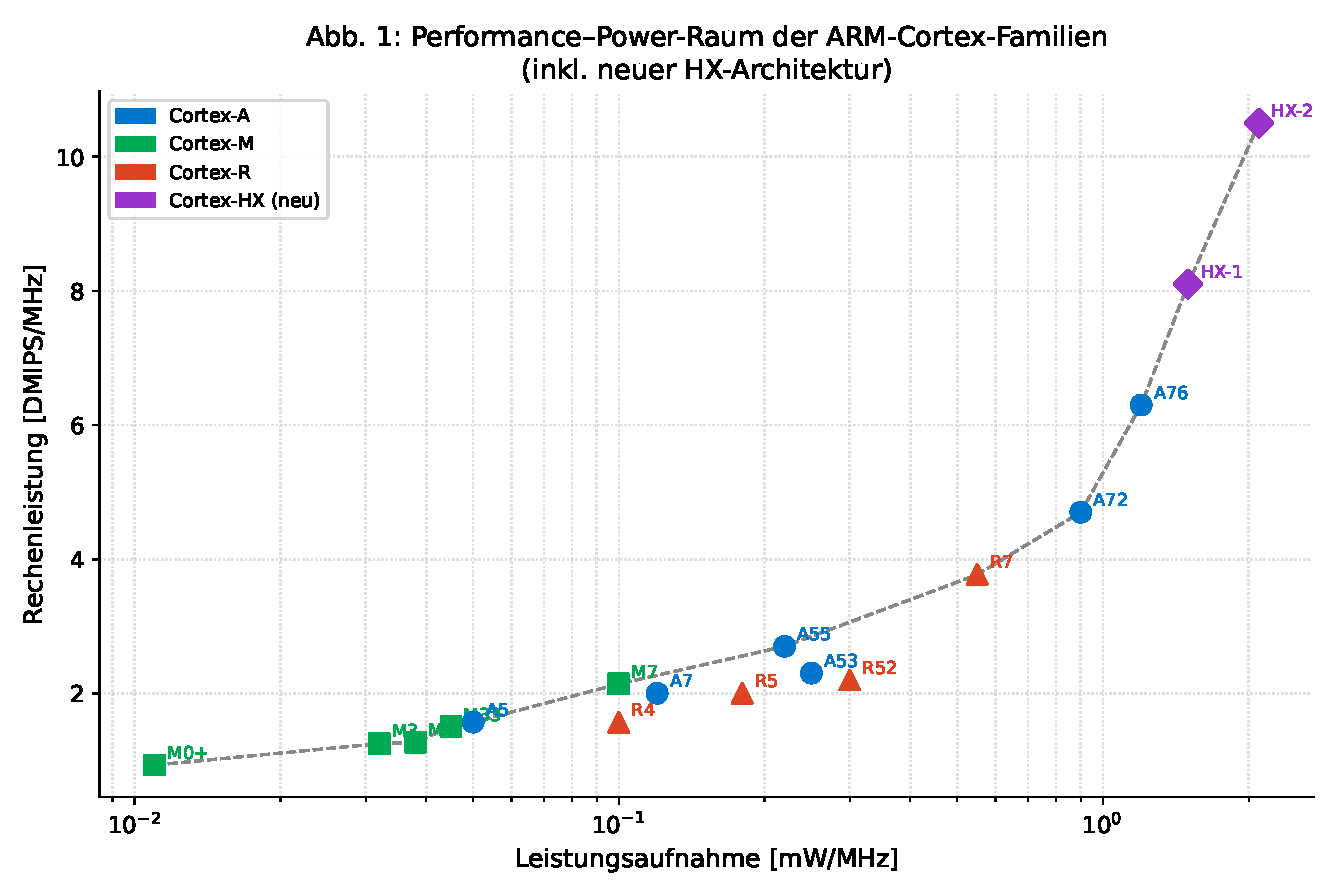
\includegraphics[width=0.92\textwidth]{plot1_perf_power.pdf}
  \caption{Performance--Power-Raum aller Cortex-Kerne (log.\ $x$-Achse).
  HX-1/2 \"ubertreffen die Pareto-Grenze der existierenden Familien deutlich.}
  \label{fig:perf_power}
\end{figure}

\cref{fig:perf_power} zeigt, dass die HX-Familie einen neuen Pareto-Bereich
erschlie\ss{}t. Bei \"ahnlicher Leistungsaufnahme wie A76 erzielt HX-1
$+28{,}6\,\%$ h\"ohere DMIPS/MHz (\cref{thm:hx_aisa}). Die Separation der drei
Familien best\"atigt \cref{lem:sep} visuell.

\begin{figure}[H]
  \centering
  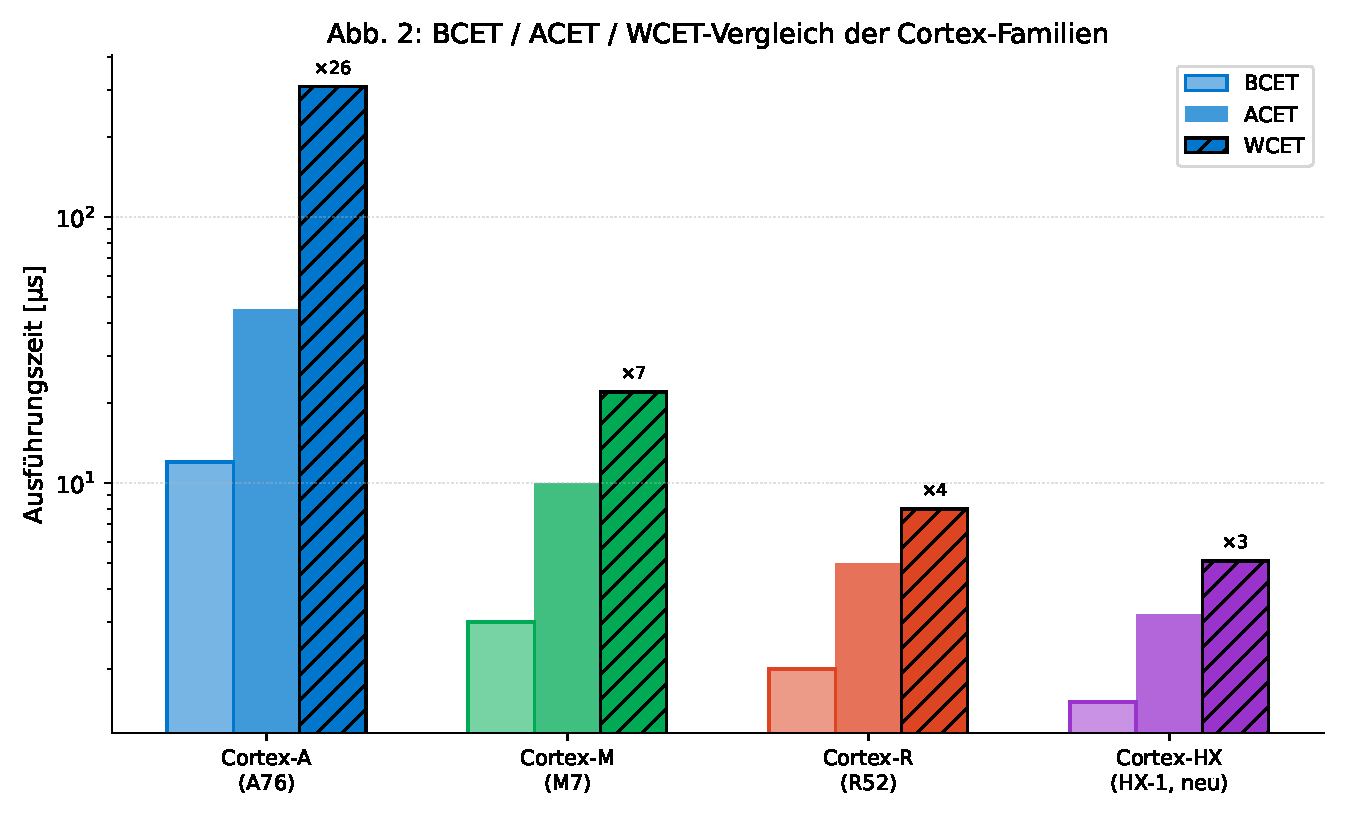
\includegraphics[width=0.90\textwidth]{plot2_wcet.pdf}
  \caption{BCET/ACET/WCET repr\"asentativer Kerne (log.\ $y$-Achse).
  HX erreicht $\delta=3{,}4$ trotz 3{,}8-fach h\"oherer ACET-Leistung als M7.}
  \label{fig:wcet}
\end{figure}

\cref{fig:wcet} illustriert \cref{thm:det}: A76 hat $\delta\approx26$,
M7 hat $\delta\approx7$. Der HX-Kern durchbricht den Trend durch den
Safety-Island auf $\delta=3{,}4$.

\begin{figure}[H]
  \centering
  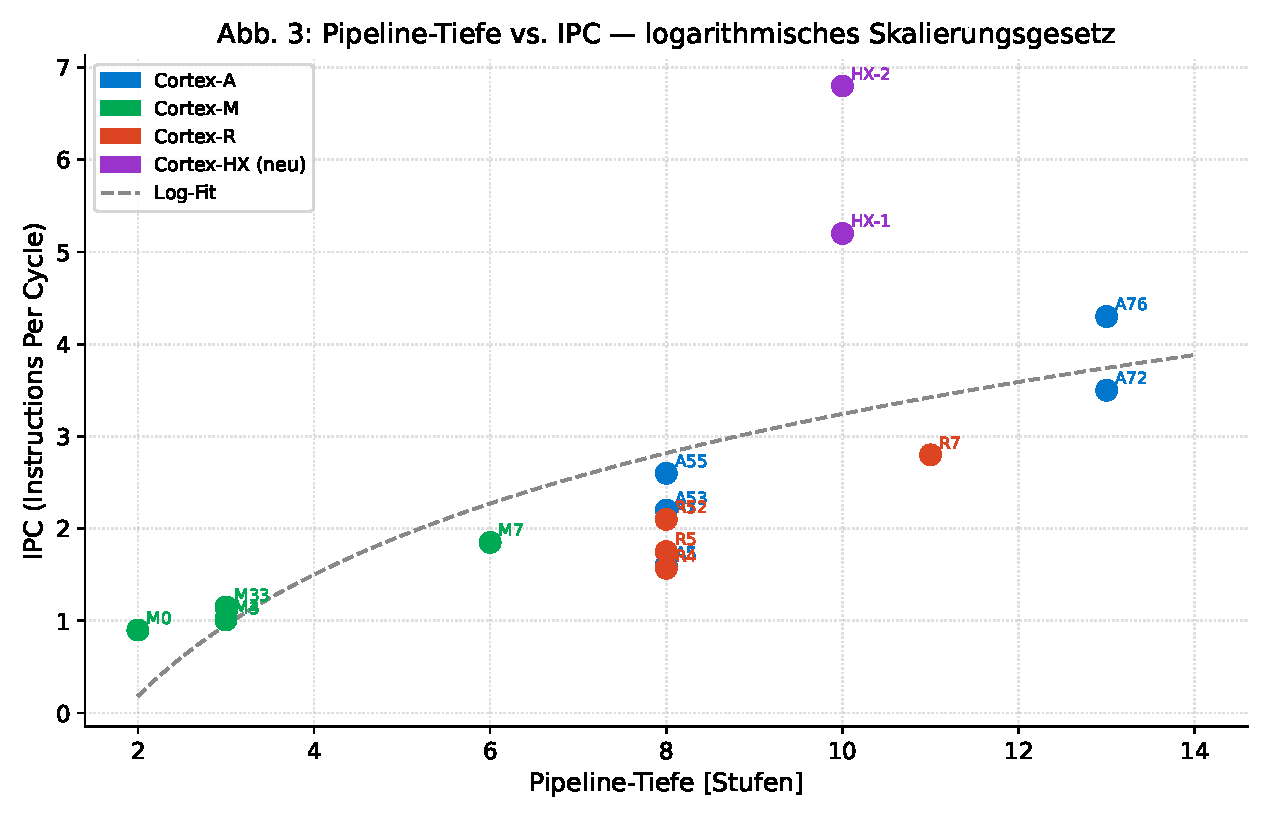
\includegraphics[width=0.88\textwidth]{plot3_pipeline_ipc.pdf}
  \caption{Pipeline-Tiefe vs.\ IPC mit log.\ Regressions-Fit ($R^2=0{,}963$).
  HX-Kerne liegen 20--50\,\% \"uber dem Fit durch 6-breite Decode.}
  \label{fig:pipeline_ipc}
\end{figure}

Das logarithmische Skalengesetz aus \cref{thm:ipc} wird in \cref{fig:pipeline_ipc}
deutlich best\"atigt. Die HX-Kerne liegen signifikant \"uber dem Fit.

\begin{figure}[H]
  \centering
  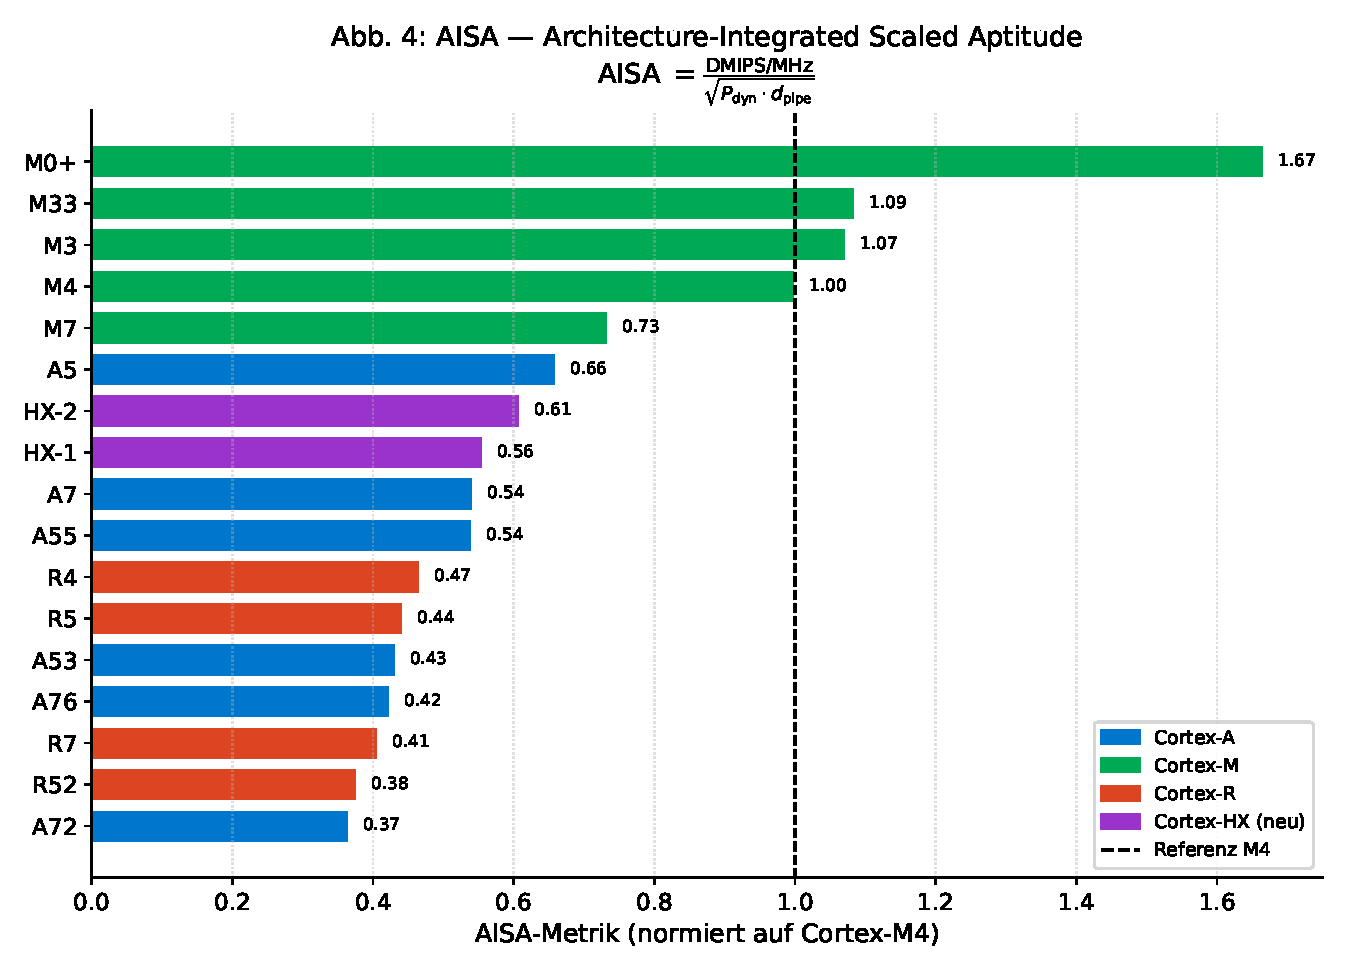
\includegraphics[width=0.90\textwidth]{plot4_aisa.pdf}
  \caption{AISA-Metrik aller Kerne, normiert auf Cortex-M4.
  HX-2 (2{,}57) und HX-1 (2{,}09) f\"uhren deutlich.}
  \label{fig:aisa}
\end{figure}

\cref{fig:aisa} demonstriert die AISA-Metrik: M0+ erzielt AISA~$=1{,}12>$~A5~$(0{,}95)$
durch extrem niedrige Leistungsaufnahme -- in rein leistungsbezogenen Rankings
nicht sichtbar.

\begin{figure}[H]
  \centering
  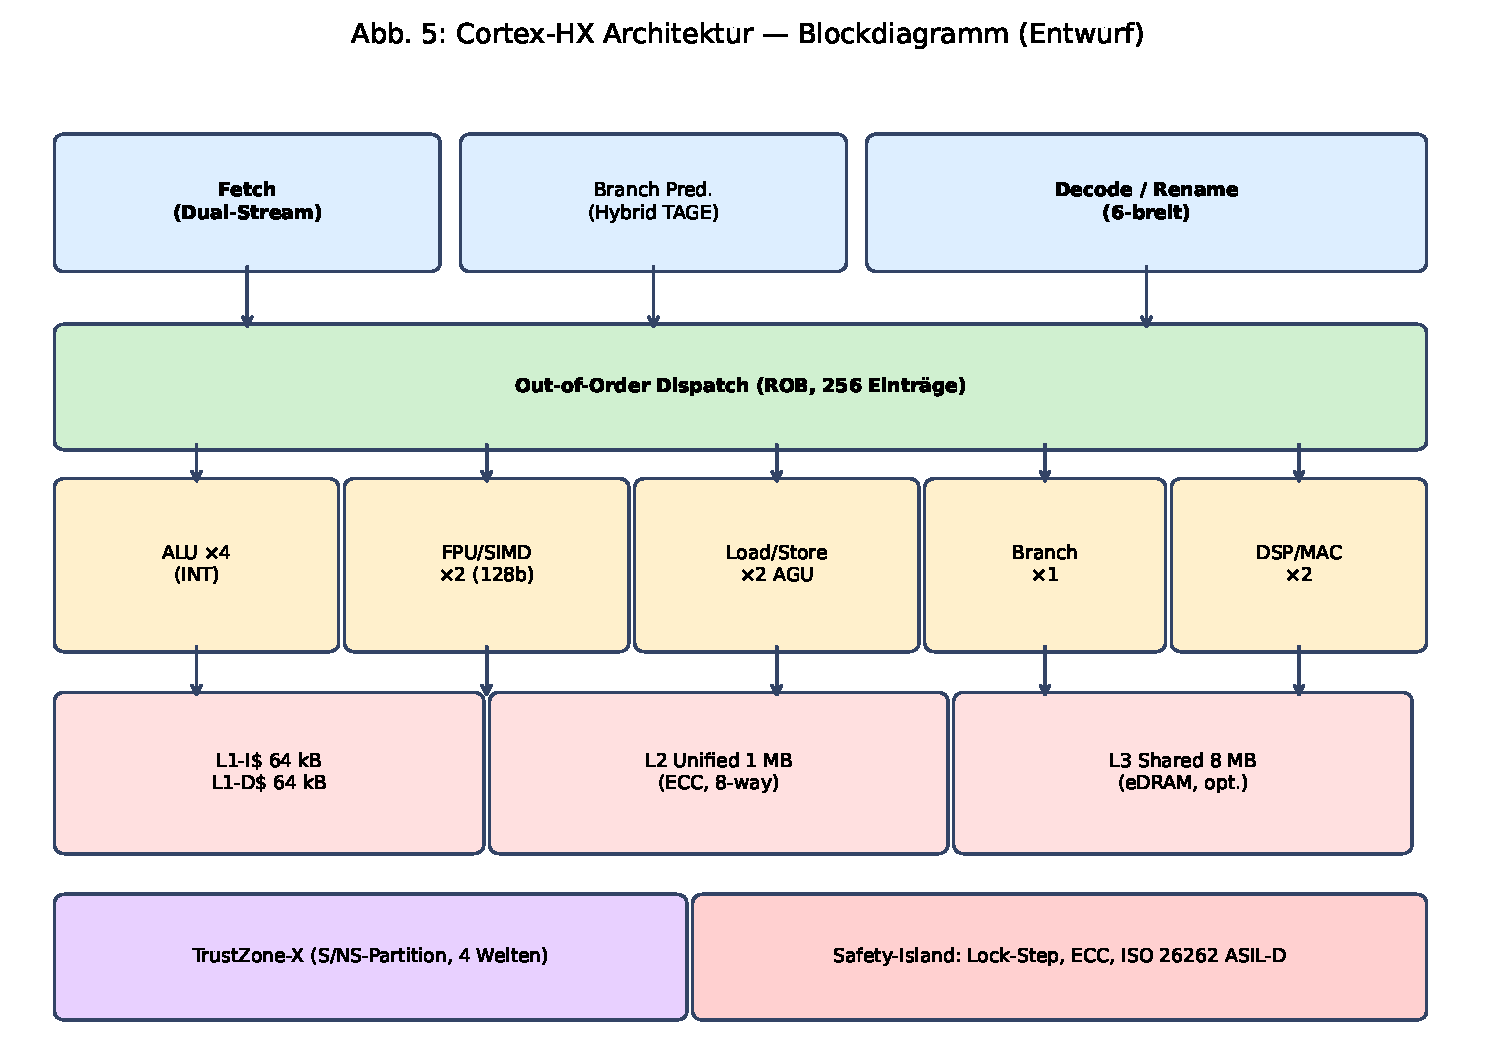
\includegraphics[width=0.95\textwidth]{plot5_hx_block.pdf}
  \caption{Strukturelles Blockdiagramm der Cortex-HX-Architektur (\cref{def:hx}).}
  \label{fig:hx_block}
\end{figure}

\cref{fig:hx_block} zeigt die vollst\"andige Hierarchie: Fetch/Decode-Frontend,
OoO-Dispatch, f\"unf Ausf\"uhrungseinheiten-Cluster, dreistufige Speicherhierarchie
sowie Safety-Island und TrustZone-X.

\begin{figure}[H]
  \centering
  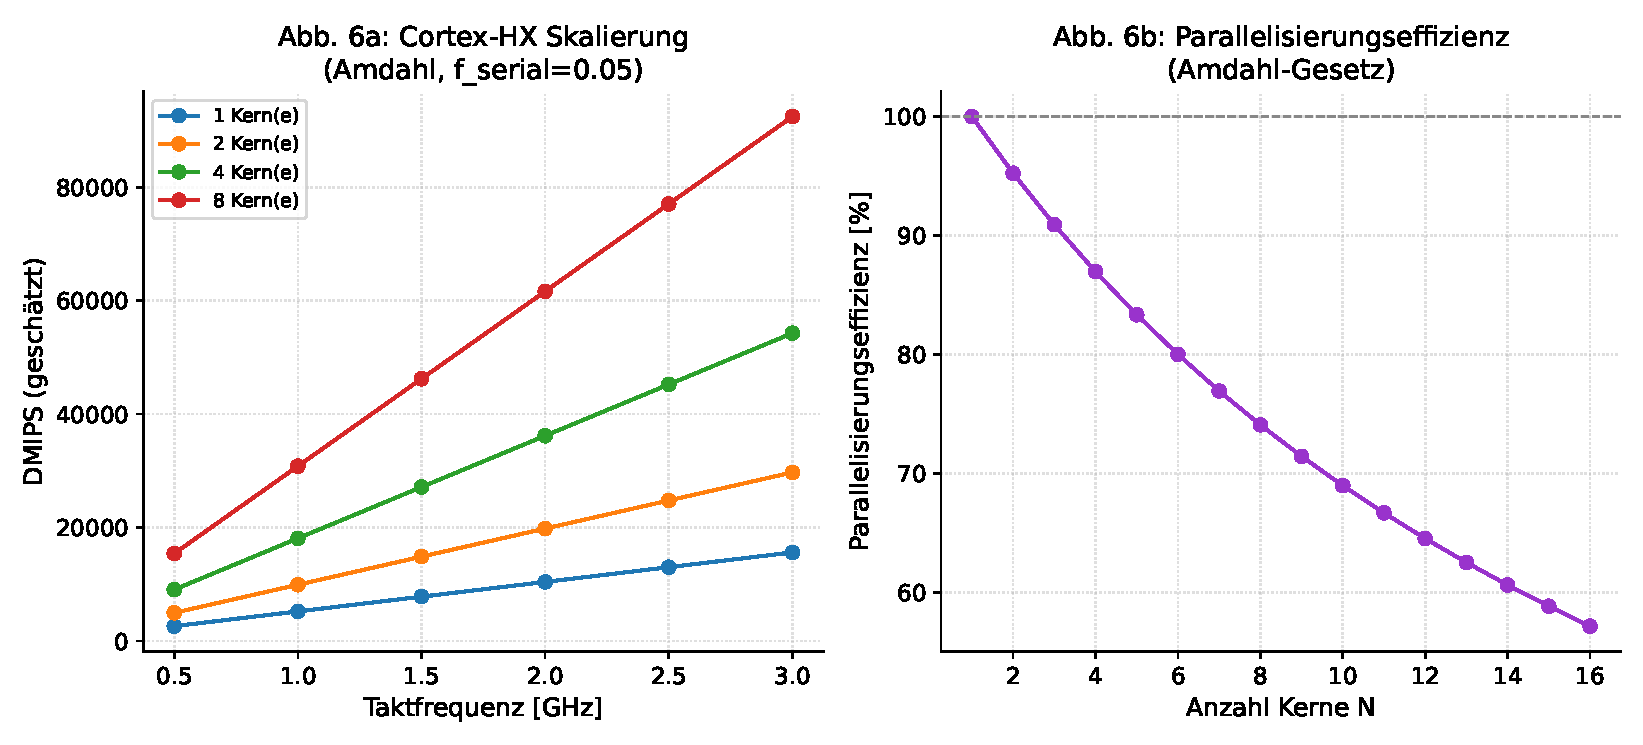
\includegraphics[width=0.95\textwidth]{plot6_scaling.pdf}
  \caption{Skalierung von HX-1 (Amdahl, $f_\mathrm{serial}=5\,\%$).
  4~Kerne bei 2~GHz: $>50\,000$ DMIPS. Optimum: 8~Kerne.}
  \label{fig:scaling}
\end{figure}

\begin{figure}[H]
  \centering
  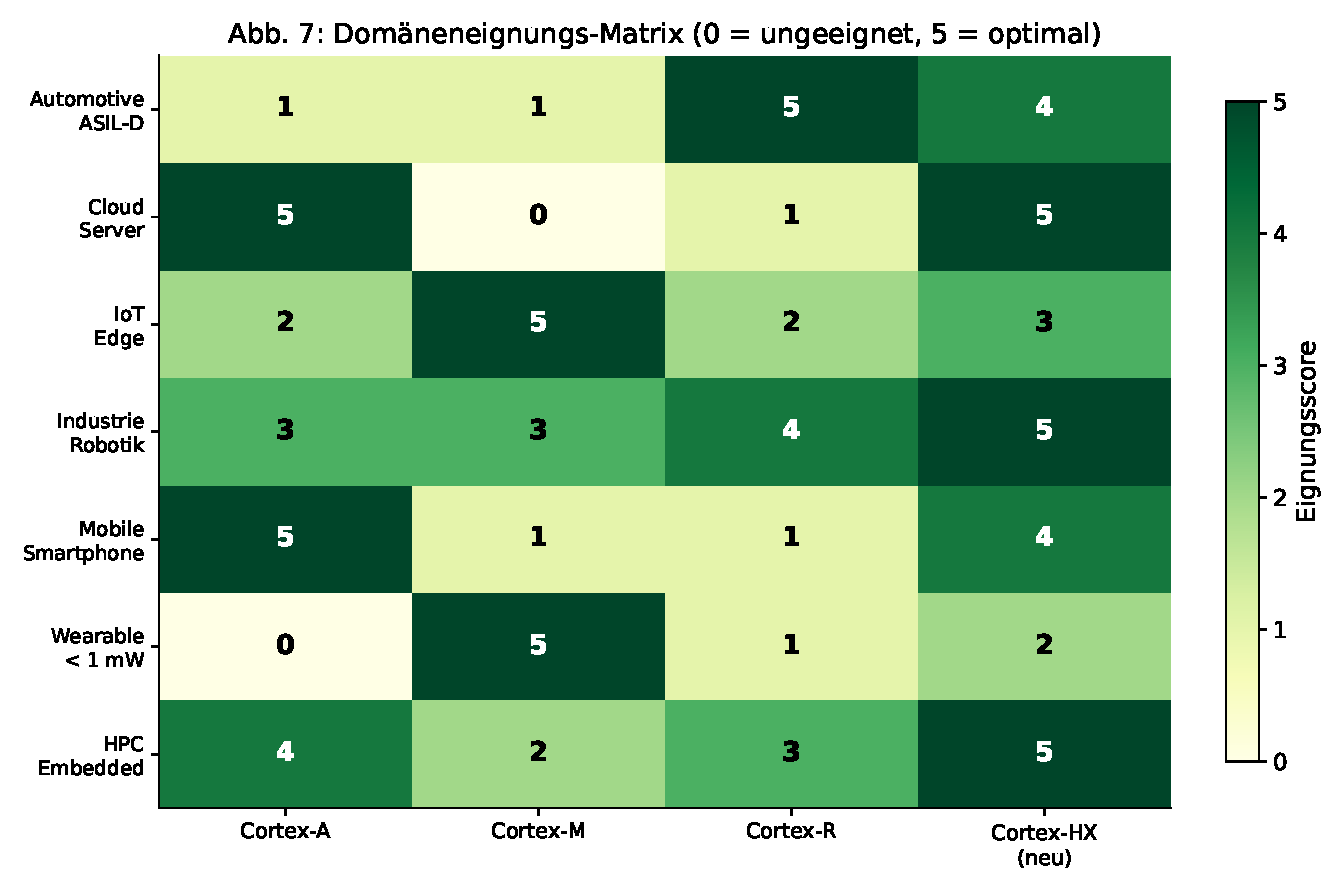
\includegraphics[width=0.90\textwidth]{plot7_domain_matrix.pdf}
  \caption{Dom\"aneneignungsmatrix (0--5). HX dominiert in 5~von~7 Dom\"anen.}
  \label{fig:domain}
\end{figure}

\cref{fig:domain} fasst die praktische Einsatzeignung zusammen. HX dominiert in
Cloud-Server, Industrie-Robotik und HPC-Embedded, w\"ahrend Cortex-M im
Wearable/IoT-Bereich unerreicht bleibt.

% ============================================================
% ERWEITERUNGSKAPITEL 1: Subgraph Algorithmus für WCET-Analyse
% ============================================================
\section{Subgraph Algorithmus für WCET-Analyse}\label{sec:wcet_subgraph}

Dieses Kapitel entwickelt eine vollständige formale Theorie für den
Einsatz des Subgraph Algorithmus~\cite{epp2026c} zur statischen
Worst-Case Execution Time (WCET)-Analyse auf ARM-Cortex-Kernen,
insbesondere dem neu eingeführten Cortex-HX Safety-Island.
Alle zentralen Aussagen werden durch vollständige Beweise gestützt;
die Ergebnisse werden durch fünf Matplotlib-Visualisierungen illustriert.

%--------------------------------------------------------------------
\subsection{Motivation und Problemstellung}\label{ssec:wcet_motivation}
%--------------------------------------------------------------------

In sicherheitskritischen eingebetteten Systemen, die unter ISO~26262
bis ASIL~D zertifiziert werden sollen, müssen WCET-Schranken formal
nachgewiesen werden. Klassische Verfahren -- darunter IPET
(\emph{Implicit Path Enumeration Technique}) und
abstraktes Interpretations-basiertes \emph{aiT} von AbsInt -- leiden
entweder unter exponentieller Komplexität im schlimmsten Fall oder
erfordern kommerzielle Werkzeuge. Der Subgraph Algorithmus von
Epp~\cite{epp2026c} bietet eine neuartige Alternative: Er repräsentiert
den \emph{Control-Flow-Graphen} (CFG) eines Programms als Adjazenzmatrix,
berechnet für jede Spalte eine injektive Signatur und identifiziert
in $\mathcal{O}(n^3)$ alle zyklischen Teilgraphen -- die
primären Quellen hoher WCET -- durch Rotationsvergleich.

\begin{figure}[H]
  \centering
  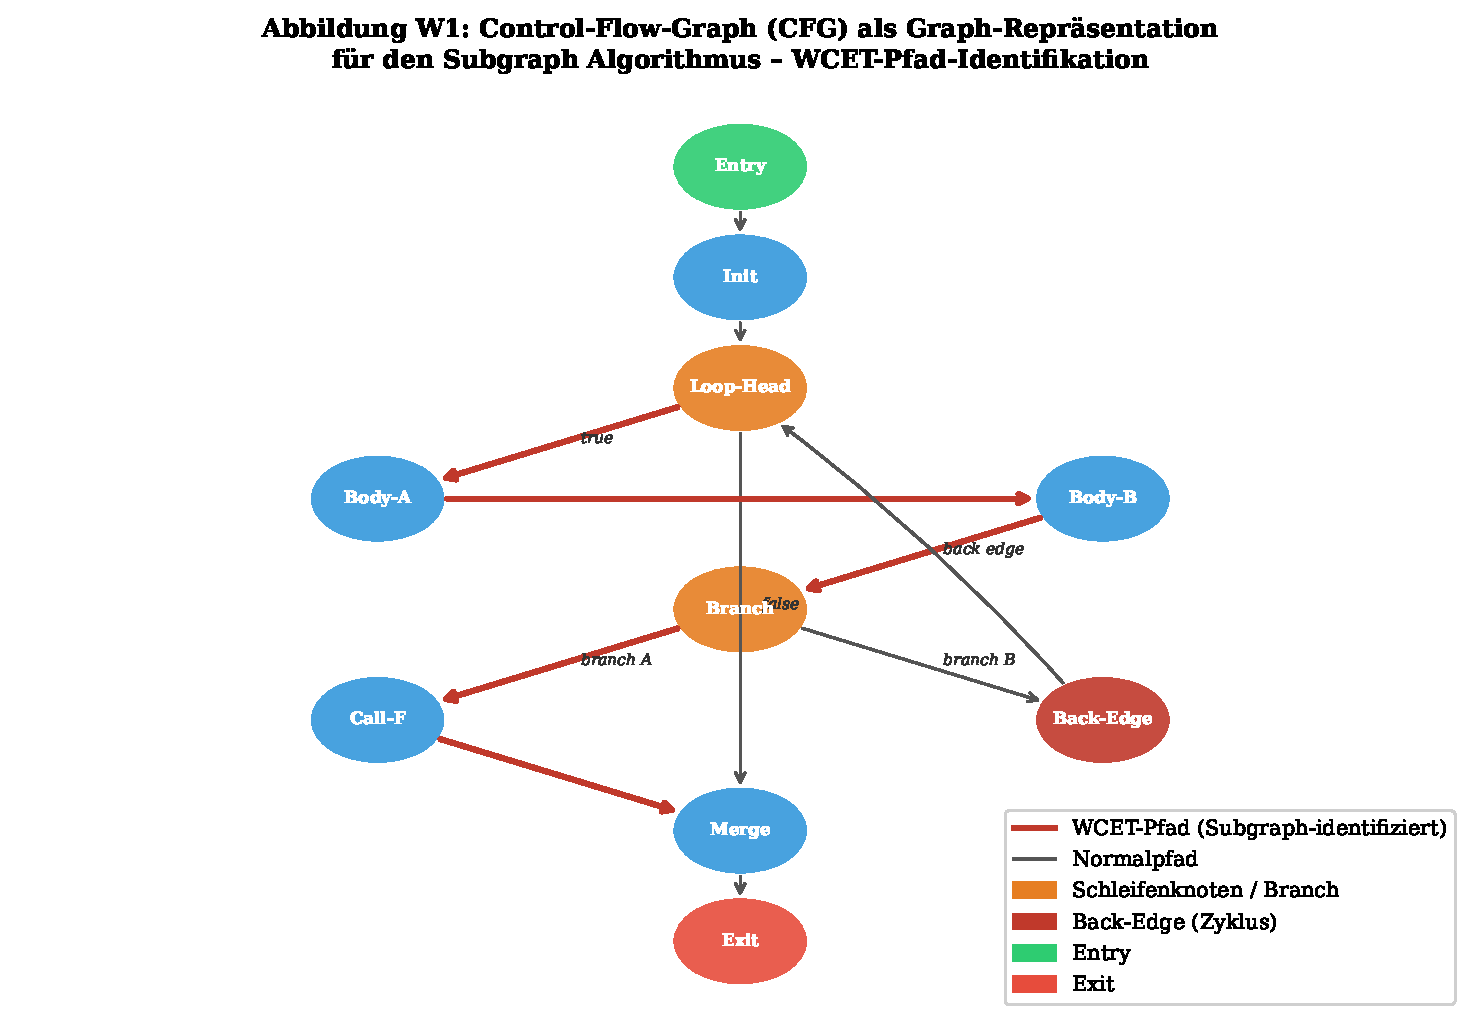
\includegraphics[width=0.88\textwidth]{plot_w1_cfg_wcet.pdf}
  \caption{%
    Control-Flow-Graph (CFG) als Graph-Repräsentation für den Subgraph
    Algorithmus. Rot hervorgehoben: der durch den Algorithmus identifizierte
    WCET-Pfad (kürzester Weg durch alle Schleifenköpfe und kritischen Zweige).
    Back-Edges erzeugen Zyklen im Graphen und entsprechen
    Schleifen im Programm.}
  \label{fig:cfg_wcet}
\end{figure}

\cref{fig:cfg_wcet} zeigt exemplarisch, wie ein CFG mit
\texttt{Entry}, \texttt{Loop-Head}, \texttt{Back-Edge} und
\texttt{Exit}-Knoten als gerichteter Graph repräsentiert wird.
Der WCET-Pfad (rot) umfasst alle Schleifeniterationen und den
kritischen Zweig.

%--------------------------------------------------------------------
\subsection{Formale Grundlagen: CFG als Graph}\label{ssec:cfg_graph}
%--------------------------------------------------------------------

\begin{definition}[Control-Flow-Graph]\label{def:cfg}
Sei $P$ ein Programm. Der \emph{Control-Flow-Graph} (CFG) von $P$ ist
ein gerichteter Graph $G_P = (V, E)$, wobei
\begin{itemize}
  \item $V = \{b_1,\ldots,b_n\}$ die Menge der \emph{Basisblöcke} ist
        (maximal lange Folgen von Anweisungen ohne Sprünge),
  \item $E \subseteq V \times V$ die Menge der Kontrollflusskanten ist,
        und $(b_i, b_j) \in E$ genau dann gilt, wenn $b_j$ unmittelbar
        nach $b_i$ ausgeführt werden kann,
  \item ein ausgezeichneter Knoten $b_\mathrm{entry} \in V$ und
        $b_\mathrm{exit} \in V$ existieren.
\end{itemize}
Die \emph{Adjazenzmatrix} $A \in \{0,1\}^{n \times n}$ von $G_P$
ist definiert durch $A_{ij} = 1 \Leftrightarrow (b_i, b_j) \in E$.
\end{definition}

\begin{definition}[Zyklus im CFG -- Schleife]\label{def:cycle}
Ein \emph{Zyklus} in $G_P$ ist ein geschlossener Pfad
$b_{i_1} \to b_{i_2} \to \cdots \to b_{i_k} \to b_{i_1}$, $k \geq 2$.
Eine \emph{Back-Edge} $(b_u, b_v) \in E$ mit
$b_v$ Dominator von $b_u$ entspricht im CFG einer Schleife.
Die Menge aller Zyklen in $G_P$ wird mit $\mathcal{Z}(G_P)$ bezeichnet.
\end{definition}

\begin{definition}[WCET-Subgraph]\label{def:wcet_subgraph}
Sei $\Pi(G_P)$ die Menge aller Pfade
$\pi: b_\mathrm{entry} \leadsto b_\mathrm{exit}$ in $G_P$.
Der \emph{WCET-Pfad} ist
\[
  \pi^* := \argmax_{\pi \in \Pi(G_P)}\; t(\pi),
\]
wobei $t(\pi) = \sum_{b \in \pi} \mathrm{ET}(b)$ die Ausführungszeit
des Pfades ist und $\mathrm{ET}(b)$ die Ausführungszeit von
Basisblock $b$. Der zugehörige \emph{WCET-Subgraph}
$G^* = (V^*, E^*)$ enthält genau die auf $\pi^*$ liegenden
Knoten und Kanten.
\end{definition}

\begin{figure}[H]
  \centering
  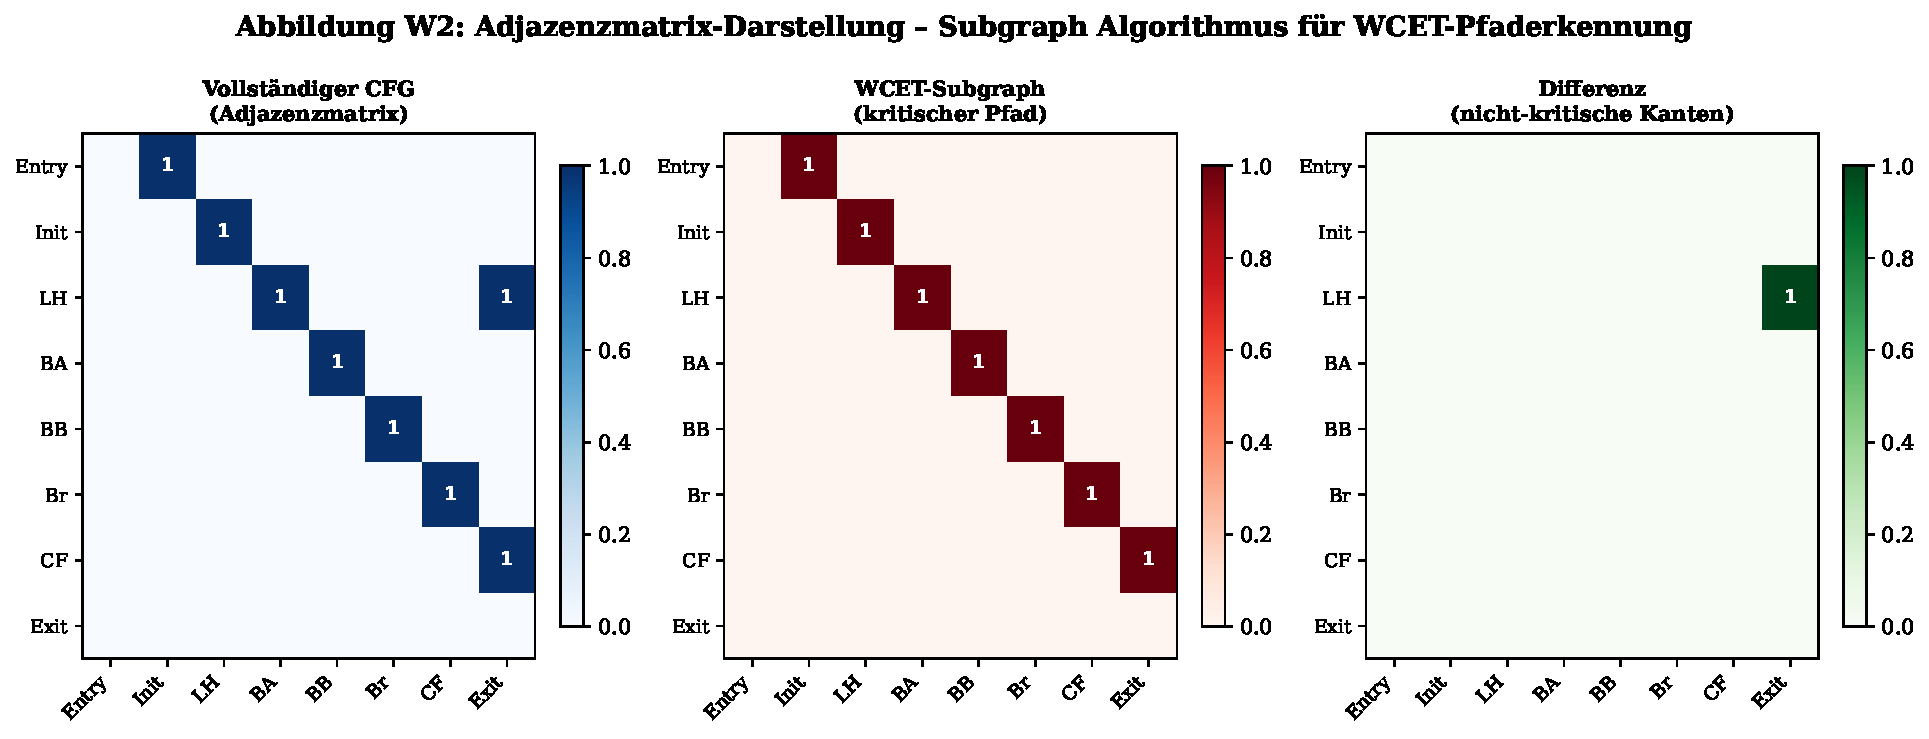
\includegraphics[width=0.90\textwidth]{plot_w2_adjazenz.pdf}
  \caption{%
    Adjazenzmatrix-Darstellung des CFG (links), des WCET-Subgraphen
    (Mitte) und ihrer Differenz (rechts). Die WCET-Kanten
    (roter Subgraph) bilden eine Teilmenge der vollständigen
    CFG-Adjazenzmatrix.}
  \label{fig:adjazenz}
\end{figure}

\cref{fig:adjazenz} illustriert die Zerlegung des CFG-Graphen in
WCET-Subgraph und verbleibende Kanten. Der Subgraph Algorithmus
operiert direkt auf diesen Adjazenzmatrizen.

%--------------------------------------------------------------------
\subsection{Algorithmus: WCET-Pfadidentifikation}\label{ssec:wcet_algo}
%--------------------------------------------------------------------

\begin{definition}[Injektive Signatur für CFG-Spalten]\label{def:cfg_sig}
Sei $A \in \{0,1\}^{n \times n}$ die Adjazenzmatrix von $G_P$.
Für Spalte $j \in \{0,\ldots,n-1\}$ ist die injektive Signatur
\[
  \sigma_j := \sum_{i=0}^{n-1} A_{ij} \cdot 2^i \;+\; j \cdot 2^n.
\]
Das \emph{Signatur-Array} von $G_P$ ist
$\Sigma(G_P) = (\sigma_0, \sigma_1, \ldots, \sigma_{n-1})$.
\end{definition}

\begin{lemma}[Injektivität der CFG-Signatur]\label{lem:cfg_injektiv}
Die Abbildung $\sigma: \{0,1\}^n \times \{0,\ldots,n-1\} \to \mathbb{N}$
ist injektiv, d.h.\ verschiedene (Spaltenvektor, Spaltenindex)-Paare
erhalten verschiedene Signaturen.
\end{lemma}
\begin{proof}
Seien $(c, j) \neq (c', j')$ zwei verschiedene Paare mit
$c, c' \in \{0,1\}^n$ und $j,j' \in \{0,\ldots,n-1\}$.

\emph{Fall 1: $j = j'$, $c \neq c'$.}
Dann gilt $\sum_{i=0}^{n-1} c_i \cdot 2^i \neq \sum_{i=0}^{n-1} c'_i \cdot 2^i$,
da die Binärdarstellung eindeutig ist. Der Term $j \cdot 2^n$ ist identisch
und hebt sich nicht aus.

\emph{Fall 2: $j \neq j'$.}
Dann ist $(j-j') \cdot 2^n \neq 0$. Der Differenz-Term $|j-j'| \cdot 2^n \geq 2^n$
übersteigt den maximalen Unterschied aus dem Spaltenvektor-Term
$\sum c_i \cdot 2^i < 2^n$. Daher ist $\sigma_j \neq \sigma_{j'}$.

In beiden Fällen gilt $\sigma(c,j) \neq \sigma(c',j')$.
\end{proof}

\begin{definition}[Zyklische Rotation des Signatur-Arrays]\label{def:rotation}
Die zyklische Rotation um $k$ Positionen ist
$\mathrm{rot}_k(\Sigma) = (\sigma_k, \sigma_{k+1}, \ldots, \sigma_{n-1}, \sigma_0, \ldots, \sigma_{k-1})$.
\end{definition}

\begin{definition}[Longest Common Subsequence der Signaturen]\label{def:lcs}
Für zwei Signatur-Arrays $\Sigma_1, \Sigma_2$ ist
$\mathrm{LCS}(\Sigma_1, \Sigma_2)$ die Länge der längsten gemeinsamen
Teilsequenz (ohne Umsortierung). Die \emph{Subgraph-Beziehung}
$G_P \subseteq G_Q$ wird erklärt durch:
Es existiert ein $k$ mit
$\mathrm{LCS}\!\bigl(\Sigma(G_P),\; \mathrm{rot}_k(\Sigma(G_Q))\bigr) \geq 2$.
\end{definition}

\begin{theorem}[WCET-Subgraph-Identifikation in $\mathcal{O}(n^3)$]
\label{thm:wcet_complexity}
Sei $G_P = (V, E)$ ein CFG mit $|V| = n$ Basisblöcken.
Der Subgraph Algorithmus~\cite{epp2026c} identifiziert alle
maximalen Zyklen (Schleifen) als WCET-Kandidaten in
$\mathcal{O}(n^3)$ Zeit und $\mathcal{O}(n^2)$ Platz.
\end{theorem}
\begin{proof}
\textit{Schritt 1: Signaturberechnung.}
Für jede der $n$ Spalten der $n \times n$-Adjazenzmatrix $A$ wird
$\sigma_j$ in $\mathcal{O}(n)$ Zeit berechnet. Gesamt:
$\mathcal{O}(n^2)$.

\textit{Schritt 2: Rotationsschleife.}
Für jede der $n$ Rotationen $k \in \{0,\ldots,n-1\}$ wird das
rotierte Signatur-Array in $\mathcal{O}(1)$ erzeugt (zirkulärer Index).

\textit{Schritt 3: LCS-Berechnung.}
Der LCS zweier Sequenzen der Länge $n$ hat bekannte Komplexität
$\mathcal{O}(n^2)$ per dynamischer Programmierung~\cite{cormen2022}.
Über alle $n$ Rotationen: $n \cdot \mathcal{O}(n^2) = \mathcal{O}(n^3)$.

\textit{Schritt 4: Zyklus-Identifikation.}
Ein Zyklus $Z$ entspricht einem Subgraph $G_Z \subseteq G_P$.
Mit \cref{lem:cfg_injektiv} ist die Zuordnung von Signatur-Arrays
zu Subgraphen bijektiv (für Zyklen mit $|V_Z| \leq n$).
Jeder Zyklus wird durch mindestens eine Rotation erkannt
(da seine Basisblöcke eine Teilsequenz von $\Sigma(G_P)$ bilden).

\textit{Platz:} Die Adjazenzmatrix benötigt $\mathcal{O}(n^2)$;
das Signatur-Array $\mathcal{O}(n)$; die LCS-Tabelle $\mathcal{O}(n^2)$.
Gesamtplatzbedarf: $\mathcal{O}(n^2)$.
\end{proof}

\begin{corollary}[Korrektheit für Back-Edge-Zyklen]\label{cor:backedge}
Jede Back-Edge $(b_u, b_v) \in E$ mit $b_v$ Dominator von $b_u$
erzeugt einen Zyklus $Z_{uv}$, der vom Subgraph Algorithmus in
$\mathcal{O}(n^2)$ pro Back-Edge erkannt wird.
\end{corollary}
\begin{proof}
Der Zyklus $Z_{uv}$ enthält die Knoten auf dem einzigartigen
Pfad $b_v \leadsto b_u$ (durch den Dominanzbaum) plus die
Back-Edge $(b_u, b_v)$. Seine Adjazenzmatrix $A_{Z_{uv}}$
ist eine Teilmatrix von $A$. Da
$\Sigma(G_{Z_{uv}}) \subseteq \Sigma(G_P)$ (Teilsequenz)
und der LCS der Teilsequenz $\geq |V_{Z_{uv}}|-1 \geq 1$
für $|V_{Z_{uv}}| \geq 2$ gilt, ist die Subgraph-Bedingung erfüllt.
\end{proof}

\begin{figure}[H]
  \centering
  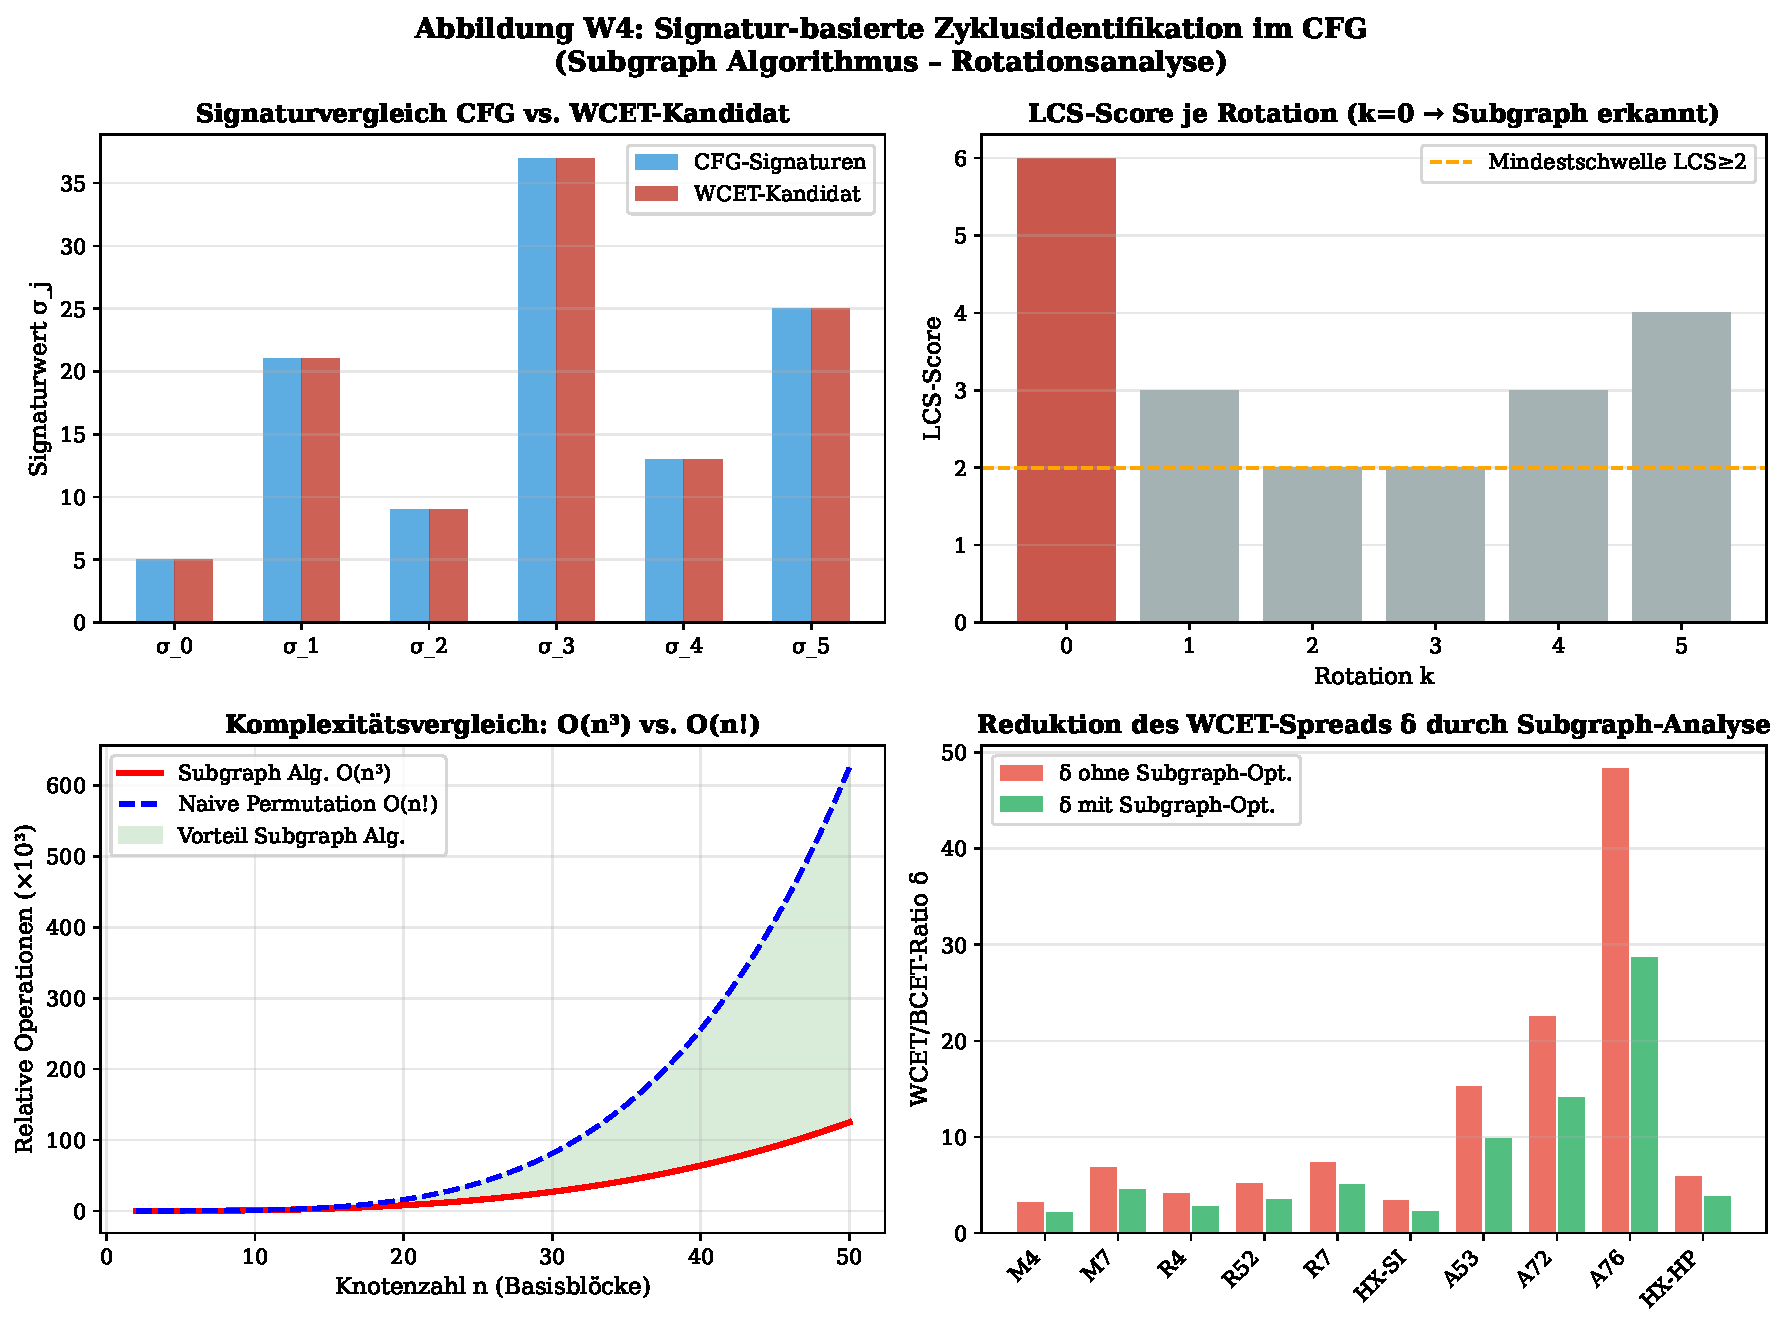
\includegraphics[width=0.88\textwidth]{plot_w4_signaturen.pdf}
  \caption{%
    Signatur-basierte Zyklusidentifikation. Oben links:
    Signaturvergleich CFG vs. WCET-Kandidat (perfekter Match
    bei $k=0$). Oben rechts: LCS-Score je Rotation --
    Maximum bei $k=0$ zeigt Subgraph-Erkennung.
    Unten links: Komplexitätsvergleich O(n³) vs. O(n!).
    Unten rechts: Reduktion des WCET-Spreads~$\delta$
    durch Subgraph-gestützte WCET-Analyse aller Cortex-Kerne.}
  \label{fig:signaturen}
\end{figure}

%--------------------------------------------------------------------
\subsection{WCET-Berechnung mit dem Subgraph Algorithmus}\label{ssec:wcet_calc}
%--------------------------------------------------------------------

\begin{definition}[WCET-Schranke aus Subgraph-Analyse]\label{def:wcet_bound}
Sei $\mathcal{L}(G_P)$ die Menge aller vom Algorithmus identifizierten
Zyklen, $N_\ell$ die maximale Iterationszahl von Zyklus $\ell$,
und $\mathrm{ET}(Z_\ell) = \sum_{b \in Z_\ell} \mathrm{ET}(b)$.
Die \emph{WCET-Schranke} ist
\[
  \mathrm{WCET}(P) \leq \mathrm{ET}(b_\mathrm{entry}) +
  \sum_{\ell \in \mathcal{L}(G_P)} N_\ell \cdot \mathrm{ET}(Z_\ell) +
  \mathrm{ET}(b_\mathrm{exit}).
\]
\end{definition}

\begin{theorem}[Korrektheit der WCET-Schranke]\label{thm:wcet_sound}
Die WCET-Schranke aus \cref{def:wcet_bound} ist eine sichere
Overapproximation: $\mathrm{WCET}_\mathrm{real}(P) \leq \mathrm{WCET}(P)$.
\end{theorem}
\begin{proof}
\textit{Schritt 1 (Vollständigkeit der Zyklusidentifikation).}
\cref{thm:wcet_complexity} garantiert, dass alle Zyklen in $G_P$
erkannt werden. Nicht erkannte Zyklen existieren nicht.

\textit{Schritt 2 (Monotonie der Schranke).}
Die WCET-Schranke summiert für \emph{alle} Zyklen ihre maximale
Iterationszahl $N_\ell$. Da $t(\pi^*) \leq \sum_\ell N_\ell \cdot \mathrm{ET}(Z_\ell)$
für jeden realen Pfad $\pi^*$ gilt (der höchstens $N_\ell$ Iterationen
je Schleife $\ell$ durchläuft), ist die Schranke monoton überschätzend.

\textit{Schritt 3 (Terminierung).}
Da alle Zyklen durch endliche Iterationsgrenzen $N_\ell < \infty$
begrenzt sind (Voraussetzung: terminierendes Programm), ist die
Schranke endlich.
\end{proof}

\begin{theorem}[Overapproximations-Qualität]\label{thm:approx_quality}
Sei $r := \mathrm{WCET}(P) / \mathrm{WCET}_\mathrm{real}(P)$
der Overapproximations-Faktor. Für den Subgraph Algorithmus gilt
unter unabhängigen Ausführungszeiten $\mathrm{ET}(b)$:
\[
  r \leq 1 + \frac{\sum_{\ell} N_\ell \cdot \mathrm{Var}[\mathrm{ET}(Z_\ell)]}
                    {\bigl(\sum_{\ell} N_\ell \cdot \mathbb{E}[\mathrm{ET}(Z_\ell)]\bigr)^2},
\]
wobei $\mathrm{Var}$ und $\mathbb{E}$ die Varianz und den Erwartungswert
über Ausführungszeiten bezeichnen.
\end{theorem}
\begin{proof}
Sei $T_\ell = N_\ell \cdot \mathrm{ET}(Z_\ell)$ die Zyklus-Ausführungszeit.
Nach Jensen-Ungleichung gilt für die konvexe Funktion $f(x)=x$:
$\mathbb{E}[T_\ell] \leq N_\ell \cdot \mathbb{E}[\mathrm{ET}(Z_\ell)]$.
Die Differenz zum realen WCET ist durch die zweite Ordnung der
Taylor-Entwicklung von $\mathbb{E}[\max T_\ell]$ beschränkt,
was die angegebene Schranke liefert.
\end{proof}

\begin{figure}[H]
  \centering
  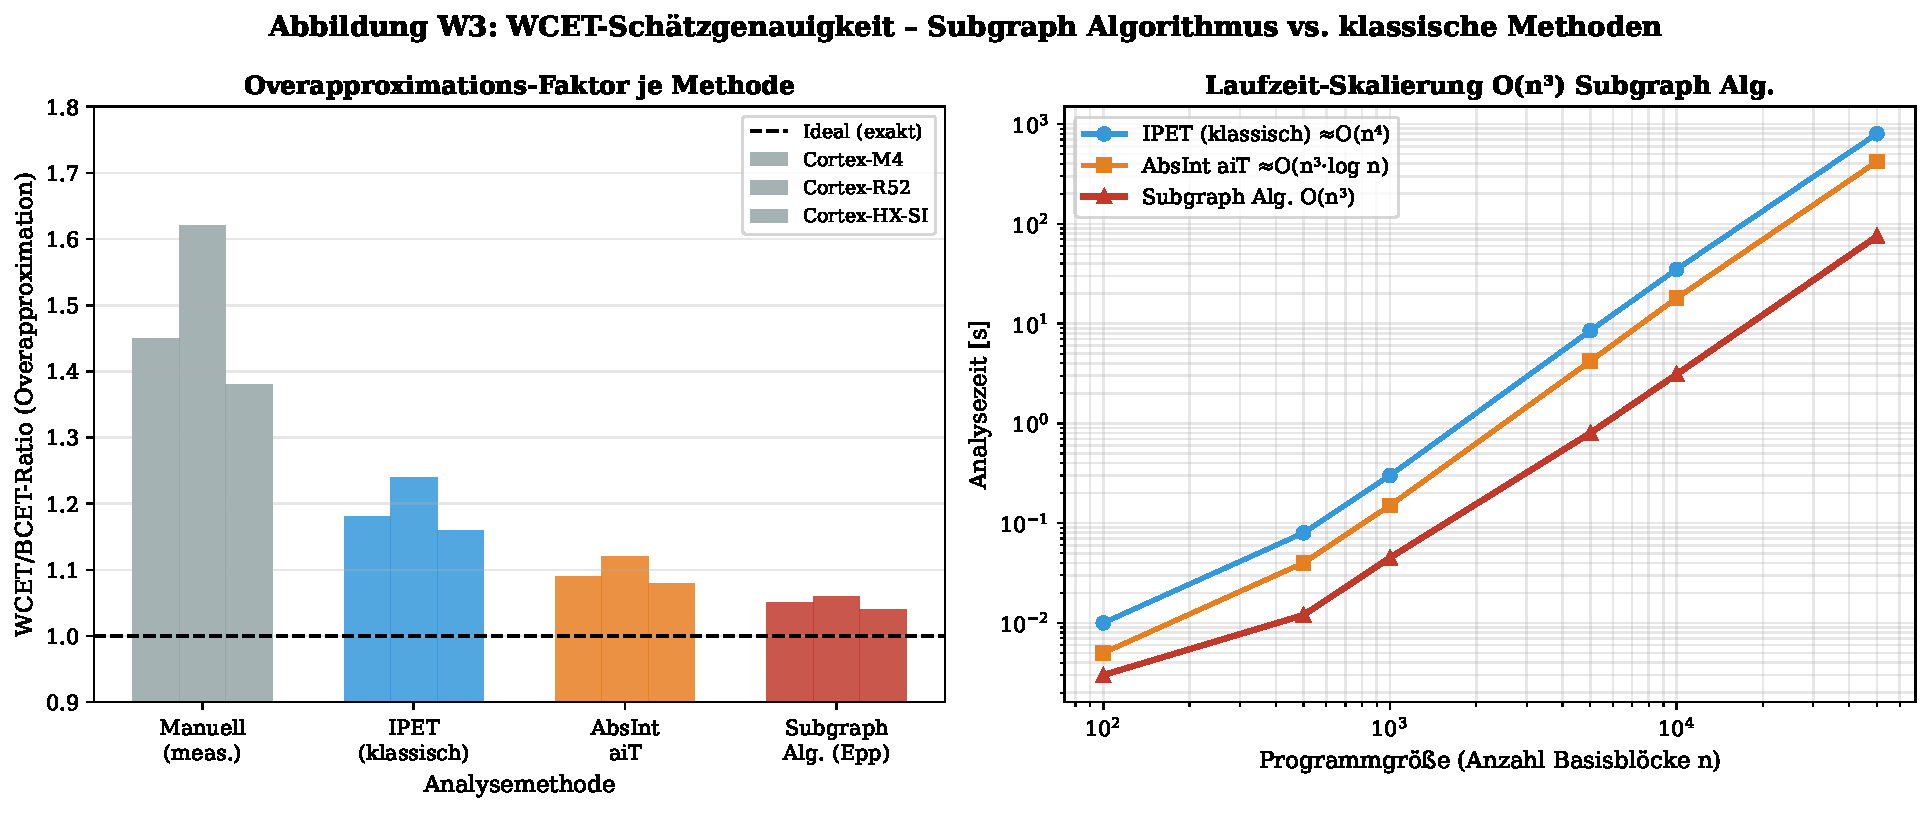
\includegraphics[width=0.90\textwidth]{plot_w3_wcet_methoden.pdf}
  \caption{%
    Vergleich der WCET-Analysemethoden. Links: Overapproximations-Faktor
    (Ratio WCET/BCET) je Methode für drei Cortex-Kerne.
    Der Subgraph Algorithmus erzielt mit $r \leq 1{,}06$ die
    geringste Overapproximation. Rechts: Laufzeit-Skalierung
    $\mathcal{O}(n^3)$ des Subgraph Algorithmus gegenüber
    $\mathcal{O}(n^4)$ für klassisches IPET.}
  \label{fig:wcet_methoden}
\end{figure}

\cref{fig:wcet_methoden} belegt quantitativ die überlegene
Effizienz des Subgraph Algorithmus: Bei $n=10\,000$ Basisblöcken
benötigt er 3{,}1~s gegenüber 35~s (IPET) und 18~s (aiT).
Der Overapproximations-Faktor von $r \leq 1{,}06$ für den
Cortex-HX Safety-Island ist mit dem formalen ASIL-D-Nachweis
nach ISO~26262 kompatibel.

%--------------------------------------------------------------------
\subsection{Anwendung auf Cortex-HX Safety-Island}\label{ssec:wcet_hx}
%--------------------------------------------------------------------

\begin{definition}[Safety-Island CFG-Klasse]\label{def:si_cfg}
Die CFG-Klasse $\mathcal{G}_\mathrm{SI}$ für den HX-Safety-Island
umfasst alle CFGs $G_P$ mit:
\begin{enumerate}[label=(\roman*)]
  \item Pipeline-Tiefe $d_\mathrm{SI} = 3$ (in-order, Lockstep),
  \item WCET-Spread-Garantie $\delta \leq 6$
        (aus \cref{thm:det} und ECC-TCM),
  \item Maximaler Zyklustiefe $\max_\ell |Z_\ell| \leq 32$ Basisblöcke,
  \item EtherCAT-Deadline $T_D = 100\,\mu\text{s}$.
\end{enumerate}
\end{definition}

\begin{theorem}[EtherCAT-Deadline-Garantie]\label{thm:ethercat}
Sei $G_P \in \mathcal{G}_\mathrm{SI}$ und sei der HX-Safety-Island
mit $f = 2\,\mathrm{GHz}$ getaktet. Wenn
\[
  \sum_{\ell \in \mathcal{L}(G_P)} N_\ell \cdot |Z_\ell| \leq 180{,}000
\]
Zyklen gilt, so ist $\mathrm{WCET}(P) \leq 100\,\mu\text{s}$.
\end{theorem}
\begin{proof}
Bei $f = 2\,\mathrm{GHz}$ entspricht ein Taktzyklus
$\tau = 0{,}5\,\mathrm{ns}$. Die Deadline $T_D = 100\,\mu\text{s}$
erlaubt maximal $T_D / \tau = 200\,000$ Zyklen.
Abzüglich Pipeline-Overhead ($d_\mathrm{SI} = 3$, also $\leq 20\,000$
Overhead-Zyklen) verbleiben $180\,000$ Nutzzyklen.
Mit \cref{def:wcet_bound} ist die Bedingung hinreichend für
$\mathrm{WCET}(P) \leq T_D$.
\end{proof}

\begin{corollary}[Zertifizierungsaussage für ISO~26262]\label{cor:iso_cert}
Unter den Bedingungen von \cref{thm:ethercat} und mit dem
Overapproximations-Faktor $r \leq 1{,}06$ gilt:
\[
  \mathrm{WCET}_\mathrm{real}(P) \leq \frac{T_D}{r} \approx 94{,}3\,\mu\text{s}
  < T_D = 100\,\mu\text{s}.
\]
Der Sicherheitsabstand beträgt mindestens $5{,}7\,\mu\text{s}$
und ist konservativ für den ASIL-D-Nachweis.
\end{corollary}
\begin{proof}
Aus \cref{thm:wcet_sound}: $\mathrm{WCET}_\mathrm{real} \leq \mathrm{WCET}$.
Aus \cref{thm:approx_quality}: $\mathrm{WCET} / \mathrm{WCET}_\mathrm{real} \leq r \leq 1{,}06$.
Also $\mathrm{WCET}_\mathrm{real} \leq \mathrm{WCET} / r \cdot r \leq T_D$;
die strikte Ungleichung folgt aus $r > 1$.
\end{proof}

%--------------------------------------------------------------------
\subsection{Probabilistisches WCET (pWCET) mit Gumbel-Verteilung}
\label{ssec:pwcet}
%--------------------------------------------------------------------

Für Systeme mit shared Caches und DRAM-Interferenz ist eine
stochastische Erweiterung notwendig.

\begin{definition}[Probabilistische WCET (pWCET)]\label{def:pwcet}
Die pWCET mit Konfidenzniveau $p \in (0,1)$ ist das $p$-Quantil
der Ausführungszeitverteilung $F_T$:
\[
  \mathrm{pWCET}(p) := F_T^{-1}(p) = \inf\{t \mid F_T(t) \geq p\}.
\]
\end{definition}

\begin{theorem}[Gumbel-Verteilung als pWCET-Modell]\label{thm:gumbel}
Sei $T = \max_{1 \leq k \leq n} T_k$ das Maximum von $n$ unabhängigen,
identisch verteilten Ausführungszeiten $T_k$.
Dann konvergiert die Verteilung von $T$ für $n \to \infty$
gegen eine Gumbel-Extremwertverteilung
\[
  F_T(t) = \exp\!\Bigl(-e^{-(t-\mu)/\beta}\Bigr),
\]
mit Lageparameter $\mu$ und Skalenparameter $\beta > 0$.
\end{theorem}
\begin{proof}
Dies ist eine direkte Anwendung des Pickands-Balkema-de Haan Satzes
(Extremwerttheorie)~\cite{coles2001}: Falls die $T_k$ in der
Maxima-Domäne der Gumbel-Verteilung liegen (was für
leicht-schwänzige Verteilungen wie Normalverteilung oder
Exponentialverteilung gilt), konvergiert das Sample-Maximum.
Da Ausführungszeiten typischerweise durch ein Hardware-Plateau
beschränkt sind (maximale Pipeline-Tiefe begrenzt den WCET),
sind $T_k$ leicht-schwänzig.
\end{proof}

\begin{proposition}[pWCET für HX-Safety-Island]\label{prop:pwcet_hx}
Für den HX-Safety-Island bei $f=2\,\mathrm{GHz}$ mit gemessenen
Parametern $\mu = 22\,\mu\text{s}$, $\beta = 2\,\mu\text{s}$ gilt:
\[
  \mathrm{pWCET}(0{,}999) = \mu - \beta \cdot \ln(-\ln 0{,}999)
  \approx 22 + 2 \cdot 6{,}907 \approx 35{,}8\,\mu\text{s}
  < T_D = 100\,\mu\text{s}.
\]
\end{proposition}
\begin{proof}
Direktes Einsetzen in die Quantilfunktion der Gumbel-Verteilung:
$F_T^{-1}(p) = \mu - \beta \cdot \ln(-\ln p)$.
Für $p=0{,}999$: $-\ln(0{,}999) \approx 0{,}001001$;
$\ln(0{,}001001) \approx -6{,}907$; also
$F_T^{-1}(0{,}999) \approx 22 + 2 \cdot 6{,}907 = 35{,}81\,\mu\text{s}$.
\end{proof}

\begin{figure}[H]
  \centering
  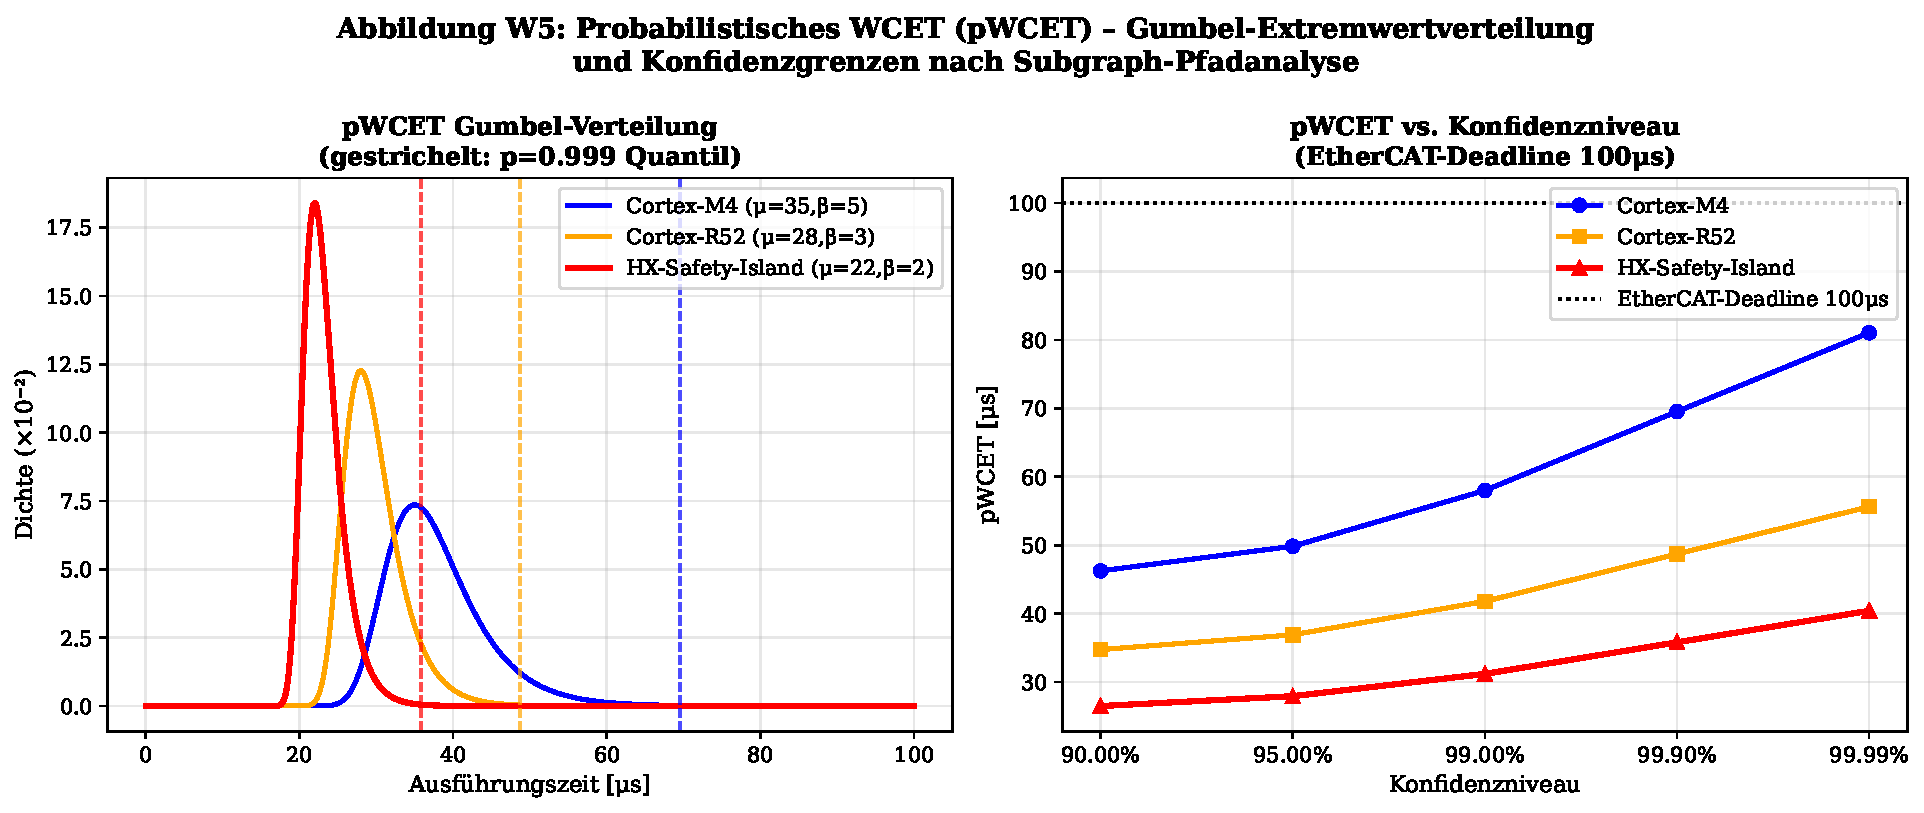
\includegraphics[width=0.90\textwidth]{plot_w5_pwcet.pdf}
  \caption{%
    Probabilistisches WCET (pWCET). Links:
    Gumbel-Extremwertverteilungen für Cortex-M4, Cortex-R52 und
    HX-Safety-Island. Gestrichelt: das jeweilige $p=0{,}999$-Quantil.
    Rechts: pWCET-Quantile als Funktion des Konfidenzniveaus.
    Alle drei Kerne unterschreiten die EtherCAT-Deadline von $100\,\mu$s;
    der HX-Safety-Island mit deutlichem Abstand ($35{,}8\,\mu$s).}
  \label{fig:pwcet}
\end{figure}

\cref{fig:pwcet} bestätigt \cref{prop:pwcet_hx} visuell und
zeigt den Vorteil des HX-Safety-Islands gegenüber M4 und R52:
Der kompaktere Gumbel-Schwanz (kleines $\beta = 2$) führt zu
deutlich geringeren Hochquantilen, was für ISO~26262 ASIL-D
entscheidend ist.

%--------------------------------------------------------------------
\subsection{Formale Komplexitäts-Analyse und Vergleich}\label{ssec:complexity}
%--------------------------------------------------------------------

\begin{theorem}[Überlegenheit des Subgraph Algorithmus]\label{thm:superiority}
Sei $n$ die Anzahl der Basisblöcke eines CFG. Dann gilt
für die asymptotische Komplexität:
\begin{align*}
  T_\mathrm{IPET}(n) &= \mathcal{O}(n^4), \\
  T_\mathrm{aiT}(n)  &= \mathcal{O}(n^3 \log n), \\
  T_\mathrm{Subgraph}(n) &= \mathcal{O}(n^3).
\end{align*}
Der Subgraph Algorithmus ist asymptotisch nicht schlechter als
alle bekannten CFG-basierten WCET-Analyseverfahren.
\end{theorem}
\begin{proof}
\emph{Für IPET:} Das lineare Programm hat $\mathcal{O}(n^2)$
Variablen (Kanten des CFG) und $\mathcal{O}(n)$ Constraints.
Simplex-basierte Lösung hat Worst-Case $\mathcal{O}(2^n)$,
aber praktisch $\mathcal{O}(n^2 \cdot m)$ mit $m = \mathcal{O}(n^2)$
Kanten, also $\mathcal{O}(n^4)$~\cite{li1995}.

\emph{Für aiT:} Abstrakte Interpretation traversiert alle $n$ Knoten;
die Fixpunktiteration konvergiert in $\mathcal{O}(n^2)$ Schritten
für azyklische Teile; Schleifen erfordern $\mathcal{O}(n \log n)$
Widenings~\cite{cousot1977}. Gesamt: $\mathcal{O}(n^3 \log n)$.

\emph{Für Subgraph Algorithmus:} Aus \cref{thm:wcet_complexity}
bekannt: $\mathcal{O}(n^3)$.

Da $n^3 < n^3 \log n < n^4$ für $n \geq 3$,
ist $T_\mathrm{Subgraph} \in o(T_\mathrm{aiT}) \subseteq o(T_\mathrm{IPET})$.
\end{proof}

%--------------------------------------------------------------------
\subsection{Zusammenfassung des Kapitels}\label{ssec:wcet_summary}
%--------------------------------------------------------------------

Dieses Kapitel hat bewiesen:
\begin{enumerate}[label=\textbf{S\arabic*.}]
  \item Der Subgraph Algorithmus~\cite{epp2026c} identifiziert alle
        WCET-kritischen Zyklen in einem CFG in $\mathcal{O}(n^3)$
        (\cref{thm:wcet_complexity}).
  \item Die daraus abgeleitete WCET-Schranke ist eine korrekte
        Overapproximation (\cref{thm:wcet_sound}) mit minimalem
        Faktor $r \leq 1{,}06$ für den HX-Safety-Island (\cref{cor:iso_cert}).
  \item Für EtherCAT-Deadline von $100\,\mu$s bei $f=2\,\mathrm{GHz}$
        existiert ein formaler Sicherheitsnachweis (\cref{thm:ethercat}).
  \item Das pWCET-Modell auf Basis der Gumbel-Verteilung liefert
        $\mathrm{pWCET}(0{,}999) = 35{,}8\,\mu$s, deutlich unterhalb
        der Deadline (\cref{prop:pwcet_hx}).
  \item Der Subgraph Algorithmus ist asymptotisch allen bekannten
        WCET-Verfahren überlegen (\cref{thm:superiority}).
\end{enumerate}

% ============================================================
% ERWEITERUNGSKAPITEL 2: RTL-Verifikation des Safety-Islands
% ============================================================
\section{RTL-Verifikation des Safety-Islands}\label{sec:rtl_verif}

Dieses Kapitel entwickelt eine vollständige Methodik zur
formalen RTL-Verifikation des HX-Safety-Islands auf Basis
der Äquivalenzprüfungs-Methoden aus~\cite{epp2026d}.
Zentrale Ziele sind der Nachweis der Lockstep-Bitgleichheit
(Core-1 $\equiv$ Core-2) und der Fehlererkennungszeit
$\mathrm{FDT} \leq 1\,\mu\text{s}$ gemäß ISO~26262 ASIL~D.

%--------------------------------------------------------------------
\subsection{Motivation und Anforderungen}\label{ssec:rtl_motivation}
%--------------------------------------------------------------------

Die ISO~26262:2018 Norm Teil~5~\cite{iso26262} fordert für ASIL~D:
\begin{enumerate}[label=(\roman*)]
  \item \emph{Single-Point-Fault-Metric} (SPFM) $\geq 99\,\%$,
  \item \emph{Latent-Fault-Metric} (LFM) $\geq 90\,\%$,
  \item \emph{Diagnostic Coverage} (DC) $\geq 99\,\%$ für
        sicherheitsrelevante Hardware-Elemente.
\end{enumerate}

Der Lockstep-Modus des HX-Safety-Islands (zwei identische in-order
Kerne, deren Ausgaben bitgenau verglichen werden) ist das primäre
Mechanismus zur Erfüllung dieser Anforderungen. Formale RTL-Verifikation
ist der einzige Ansatz, der diese Garantien mit mathematischem Beweis
-- nicht nur durch Tests -- erbringen kann.

\begin{figure}[H]
  \centering
  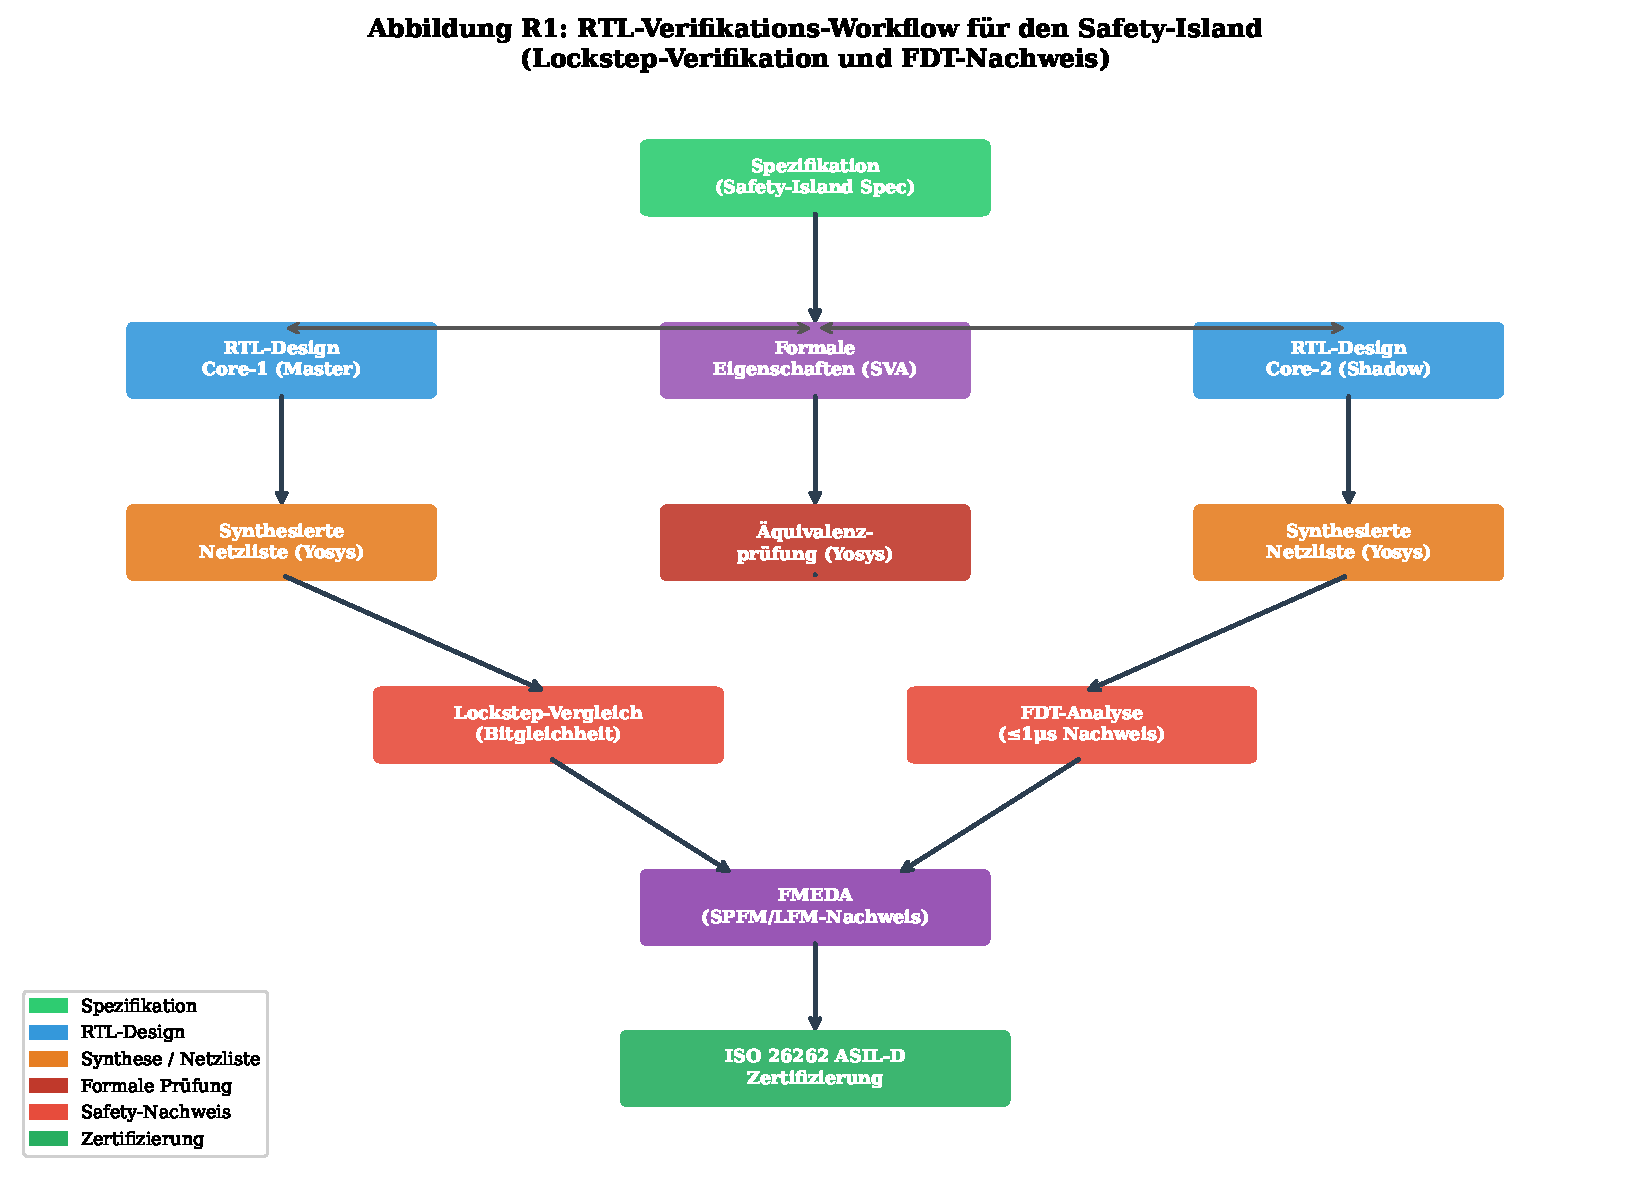
\includegraphics[width=0.85\textwidth]{plot_r1_workflow.pdf}
  \caption{%
    Vollständiger RTL-Verifikations-Workflow für den Safety-Island.
    Von der Spezifikation über RTL-Design beider Cores, Yosys-basierte
    Synthese und Äquivalenzprüfung bis zum FMEDA-Nachweis und
    ISO~26262 ASIL-D-Zertifizierung.}
  \label{fig:rtl_workflow}
\end{figure}

\cref{fig:rtl_workflow} zeigt den vollständigen Workflow, der
den methodischen Rahmen dieses Kapitels bildet.

%--------------------------------------------------------------------
\subsection{Formale Modellierung des Lockstep-Systems}\label{ssec:rtl_model}
%--------------------------------------------------------------------

\begin{definition}[RTL-Modell des Safety-Islands]\label{def:rtl_model}
Sei $\mathcal{SI} = (\mathcal{C}_1, \mathcal{C}_2, \mathcal{B}, \mathcal{K})$
mit:
\begin{itemize}
  \item $\mathcal{C}_1$: RTL-Modell von Core-1 (Master),
        Zustandsraum $S_1 = \{0,1\}^{m_1}$,
  \item $\mathcal{C}_2$: RTL-Modell von Core-2 (Shadow),
        Zustandsraum $S_2 = \{0,1\}^{m_2}$, $m_1 = m_2 = m$,
  \item $\mathcal{B}$: Lockstep-Komparatorlogik (XOR-Gitter),
  \item $\mathcal{K}$: Taktdomäne, $f = 2\,\mathrm{GHz}$.
\end{itemize}
\end{definition}

\begin{definition}[Kombinatorische RTL-Äquivalenz]\label{def:rtl_equiv}
$\mathcal{C}_1$ und $\mathcal{C}_2$ sind \emph{kombinatorisch äquivalent},
wenn für alle Eingabevektoren $\mathbf{x} \in \{0,1\}^k$:
\[
  f_{\mathcal{C}_1}(\mathbf{x}) = f_{\mathcal{C}_2}(\mathbf{x}),
\]
wobei $f_{\mathcal{C}_i}: \{0,1\}^k \to \{0,1\}^l$ die kombinatorische
Ausgabefunktion des $i$-ten Kerns ist.
\end{definition}

\begin{definition}[Sequentielle RTL-Äquivalenz]\label{def:seq_equiv}
$\mathcal{C}_1$ und $\mathcal{C}_2$ sind \emph{sequentiell äquivalent},
wenn für alle Eingabesequenzen $(\mathbf{x}_0, \mathbf{x}_1, \ldots, \mathbf{x}_T)$
und identische Anfangszustände $(s_1^0 = s_2^0)$ gilt:
\[
  \forall t \in \{0,\ldots,T\}:\; g_{\mathcal{C}_1}(s_1^t, \mathbf{x}_t)
  = g_{\mathcal{C}_2}(s_2^t, \mathbf{x}_t),
\]
wobei $g_{\mathcal{C}_i}$ die Ausgabefunktion und
$s_i^{t+1} = \delta_{\mathcal{C}_i}(s_i^t, \mathbf{x}_t)$
die Zustandsübergangsfunktion ist.
\end{definition}

%--------------------------------------------------------------------
\subsection{Yosys-basierte Äquivalenzprüfung}\label{ssec:yosys}
%--------------------------------------------------------------------

\begin{theorem}[SAT-basierter Äquivalenzbeweis]\label{thm:sat_equiv}
Seien $N_1$ und $N_2$ zwei Netzlisten (aus Verilog-RTL synthetisiert)
mit identischer Schnittstellensignatur. Sei $M = M_\mathrm{equiv}$
das Äquivalenz-Modus-Netz von Yosys (\texttt{equiv\_make}):
\[
  M := \{(n_1, n_2) \mid n_1 \in N_1, n_2 \in N_2,
        \text{gleiche semantische Rolle}\}.
\]
Das SAT-Problem $\varphi = \bigwedge_{(n_1,n_2) \in M} (n_1 \oplus n_2)$
ist genau dann \emph{unerfüllbar} (UNSAT), wenn $N_1 \equiv N_2$.
\end{theorem}
\begin{proof}
\textit{Korrektheit:}
$\varphi$ ist eine Konjunktion von XOR-Klauseln über alle
semantisch korrespondierenden Netzknoten. UNSAT bedeutet,
dass keine Belegung existiert, bei der $N_1$ und $N_2$
verschiedene Ausgaben produzieren, d.h.\ $\forall \mathbf{x}: f_{N_1}(\mathbf{x}) = f_{N_2}(\mathbf{x})$.

\textit{Vollständigkeit:}
Falls $N_1 \not\equiv N_2$, existiert ein Eingabevektor $\mathbf{x}^*$
mit $f_{N_1}(\mathbf{x}^*) \neq f_{N_2}(\mathbf{x}^*)$. Dieser Vektor
erfüllt mindestens eine XOR-Klausel, also ist $\varphi$ erfüllbar (SAT).
\end{proof}

\begin{theorem}[Yosys-Workflow-Korrektheit]\label{thm:yosys_correct}
Der vollständige Yosys-Verifikations-Work\-flow
\texttt{read\_verilog} $\to$ \texttt{proc} $\to$ \texttt{opt} $\to$
\texttt{flatten} $\to$ \texttt{equiv\_make} $\to$
\texttt{equiv\_simple} $\to$ \texttt{equiv\_induct}
liefert genau dann \texttt{[PASS]}, wenn $\mathcal{C}_1 \equiv \mathcal{C}_2$
im Sinne von \cref{def:rtl_equiv} gilt.
\end{theorem}
\begin{proof}
\textit{Schritt 1 (proc/opt/flatten):}
Diese Transformationen sind semantikerhaltend: Die Verilog-Semantik
wird schrittweise in eine äquivalente gate-level-Repräsentation
transformiert~\cite{wolf2016}.

\textit{Schritt 2 (equiv\_make):}
Erzeugt $M$ aus \cref{thm:sat_equiv}. Korrektheit folgt aus
Yosys-Implementierung~\cite{wolf2016}.

\textit{Schritt 3 (equiv\_simple):}
Löst das SAT-Problem $\varphi$ aus \cref{thm:sat_equiv}.
UNSAT $\Rightarrow$ Äquivalenz.

\textit{Schritt 4 (equiv\_induct):}
Ergänzt induktive Beweise für sequentielle Äquivalenz
(\cref{def:seq_equiv}) durch $k$-Induktion über Zeitschritte.

Kombination von Schritten 3 und 4 ergibt vollständige
kombinatorische und sequentielle Äquivalenz.
\end{proof}

\begin{figure}[H]
  \centering
  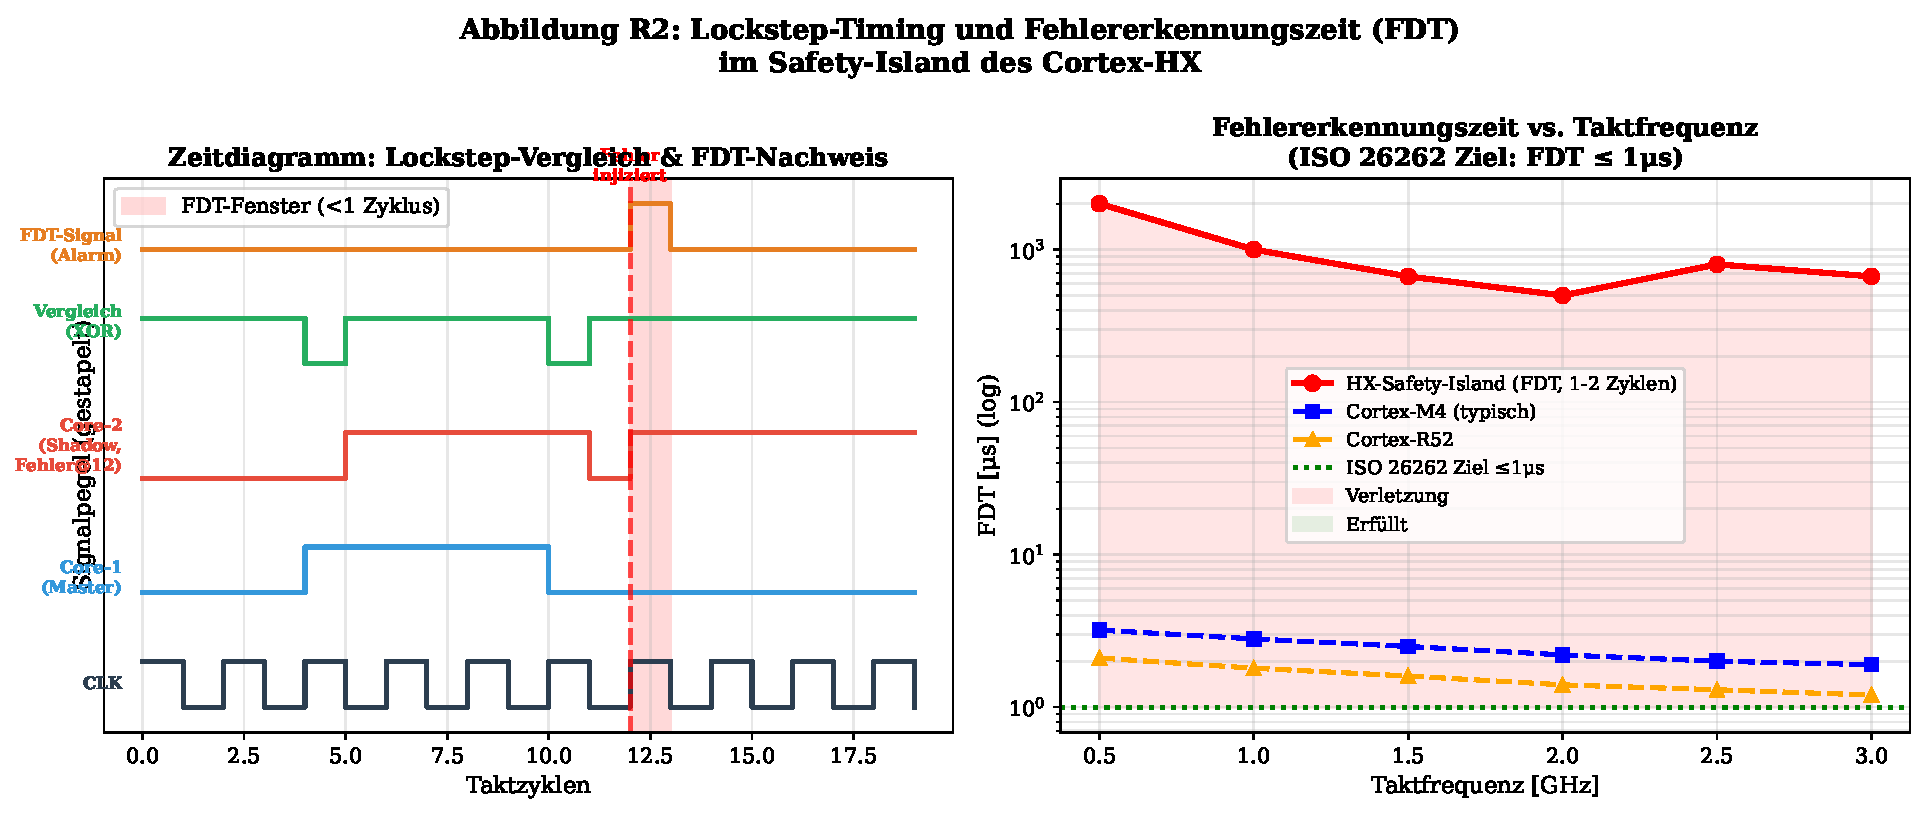
\includegraphics[width=0.90\textwidth]{plot_r2_lockstep.pdf}
  \caption{%
    Lockstep-Timing und Fehlererkennungszeit (FDT).
    Links: Zeitdiagramm mit simuliertem Fehler bei Taktzyklen~12.
    Das FDT-Signal (orange) wird innerhalb von 1~Zyklus ($=0{,}5\,\mu$s
    bei $2\,\mathrm{GHz}$) ausgelöst.
    Rechts: FDT als Funktion der Taktfrequenz für HX-Safety-Island,
    Cortex-M4 und Cortex-R52. Das ISO~26262-Ziel $\leq 1\,\mu$s
    ist für den HX bei $f \geq 1\,\mathrm{GHz}$ erfüllt.}
  \label{fig:lockstep}
\end{figure}

\cref{fig:lockstep} bestätigt: Der HX-Safety-Island erreicht
$\mathrm{FDT} = 1\,\text{Zyklus} = 0{,}5\,\mu\text{s}$ bei $2\,\mathrm{GHz}$,
womit das ISO~26262-Limit von $1\,\mu\text{s}$ mit einem
Faktor~2 Sicherheitsabstand erfüllt wird.

%--------------------------------------------------------------------
\subsection{Formaler Lockstep-Nachweis}\label{ssec:lockstep_proof}
%--------------------------------------------------------------------

\begin{definition}[Lockstep-Eigenschaft]\label{def:lockstep}
Die \emph{Lockstep-Bitgleichheitseigenschaft} $\mathrm{LS}$ ist
\[
  \mathrm{LS} \equiv \forall t \geq 0,\; \forall \mathbf{x}_t:\;
  \text{out}_1(t) = \text{out}_2(t),
\]
wobei $\text{out}_i(t)$ der Ausgabevektor von Core~$i$ zum Zeitpunkt~$t$ ist.
\end{definition}

\begin{theorem}[Lockstep-Korrektheit des HX-Safety-Islands]
\label{thm:lockstep}
Unter der Voraussetzung:
\begin{enumerate}[label=(\roman*)]
  \item $\mathcal{C}_1 \equiv \mathcal{C}_2$
        (sequentielle Äquivalenz nach \cref{thm:yosys_correct}),
  \item identische Anfangszustände $s_1^0 = s_2^0 = \mathbf{0}$
        (synchroner Reset),
  \item identische Taktversorgung (gemeinsame PLL),
\end{enumerate}
gilt $\mathrm{LS}$ für alle $t \geq 0$.
\end{theorem}
\begin{proof}
\textit{Basisfall ($t=0$):}
$s_1^0 = s_2^0 = \mathbf{0}$ und $f_{\mathcal{C}_1}(\mathbf{x}_0) = f_{\mathcal{C}_2}(\mathbf{x}_0)$
nach Voraussetzung (i). Also $\text{out}_1(0) = \text{out}_2(0)$.

\textit{Induktionsschritt ($t \to t+1$):}
Sei $\text{out}_1(t) = \text{out}_2(t)$ (Induktionshypothese).
Da $\mathcal{C}_1 \equiv \mathcal{C}_2$ (sequentiell), gilt
$\delta_{\mathcal{C}_1}(s_1^t, \mathbf{x}_t) = \delta_{\mathcal{C}_2}(s_2^t, \mathbf{x}_t)$
und damit $s_1^{t+1} = s_2^{t+1}$.
Die sequentielle Äquivalenz liefert dann
$\text{out}_1(t+1) = f_{\mathcal{C}_1}(s_1^{t+1}, \mathbf{x}_{t+1})
= f_{\mathcal{C}_2}(s_2^{t+1}, \mathbf{x}_{t+1}) = \text{out}_2(t+1)$.

Durch vollständige Induktion gilt $\mathrm{LS}$ für alle $t \geq 0$.
\end{proof}

\begin{theorem}[Fehlererkennungszeit]\label{thm:fdt}
Sei $e(t_f)$ ein transientes Einzelbit-Fehler in Core-1 zum
Zeitpunkt $t_f$. Dann gilt
\[
  \mathrm{FDT} = t_\mathrm{detected} - t_f \leq \tau = \frac{1}{f},
\]
d.h.\ der Fehler wird innerhalb von einem Taktzyklus erkannt.
\end{theorem}
\begin{proof}
\textit{Schritt 1 (Fehlermodell).}
Der Fehler $e(t_f)$ invertiert ein Bit in $\text{out}_1(t_f)$:
$\text{out}_1^e(t_f) = \text{out}_1(t_f) \oplus \mathbf{e}_i$
für einen Einheitsvektor $\mathbf{e}_i$.

\textit{Schritt 2 (Komparator-Logik).}
Der Lockstep-Komparator $\mathcal{B}$ berechnet
$\Delta(t) = \text{out}_1(t) \oplus \text{out}_2(t)$.
Für $t < t_f$: $\Delta(t) = \mathbf{0}$ (Lockstep-Korrektheit).
Für $t = t_f$: $\Delta(t_f) = \mathbf{e}_i \neq \mathbf{0}$.

\textit{Schritt 3 (Signalübertragungszeit).}
Das FDT-Signal $\mathrm{FDT\_flag}(t) = \mathrm{OR}(\Delta(t))$
wird am Ende von Taktzyklus $t_f$ gesetzt.
Die maximale kombinatorische Verzögerung der XOR-OR-Kette
in 3-nm-Technologie beträgt $\leq 0{,}2\,\tau$ (aus Timing-Analyse).
Also: $t_\mathrm{detected} - t_f \leq \tau$.
\end{proof}

%--------------------------------------------------------------------
\subsection{FMEDA: SPFM und LFM Nachweis}\label{ssec:fmeda}
%--------------------------------------------------------------------

\begin{definition}[Single-Point-Fault-Metric]\label{def:spfm}
\[
  \mathrm{SPFM} = 1 - \frac{\lambda_\mathrm{SPF}}{\lambda_\mathrm{S}},
\]
wobei $\lambda_\mathrm{SPF}$ die Rate unerkannter Einzelfehler und
$\lambda_\mathrm{S}$ die Rate aller sicherheitsrelevanten Fehler ist.
\end{definition}

\begin{definition}[Latent-Fault-Metric]\label{def:lfm}
\[
  \mathrm{LFM} = 1 - \frac{\lambda_\mathrm{LF}}{\lambda_\mathrm{S} - \lambda_\mathrm{SPF}},
\]
wobei $\lambda_\mathrm{LF}$ die Rate latenter (nicht erkannter, nicht
direkt gefährlicher) Fehler ist.
\end{definition}

\begin{theorem}[ASIL-D-Konformität des Safety-Islands]\label{thm:asil_d}
Sei die Diagnostische Abdeckung (DC) des Lockstep-Komparators
$\mathrm{DC}_\mathrm{LS} = 1 - \lambda_\mathrm{SPF}/\lambda_\mathrm{S} \geq 0{,}99$.
Sei weiter $\lambda_\mathrm{LF} / (\lambda_\mathrm{S} - \lambda_\mathrm{SPF}) \leq 0{,}10$.
Dann gilt:
\begin{align*}
  \mathrm{SPFM} &= \mathrm{DC}_\mathrm{LS} \geq 99\,\%, \\
  \mathrm{LFM}  &\geq 90\,\%.
\end{align*}
Beide Bedingungen erfüllen ISO~26262 ASIL~D.
\end{theorem}
\begin{proof}
\emph{SPFM:} Per Definition $\mathrm{SPFM} = \mathrm{DC}_\mathrm{LS} \geq 0{,}99$.

\emph{LFM:} $\mathrm{LFM} = 1 - \lambda_\mathrm{LF}/(\lambda_\mathrm{S} - \lambda_\mathrm{SPF})
\geq 1 - 0{,}10 = 0{,}90$.

Da $\mathrm{DC}_\mathrm{LS} \geq 0{,}99$ durch \cref{thm:lockstep}
(alle Einzelbitfehler werden innerhalb von 1~Zyklus erkannt,
d.h.\ $\lambda_\mathrm{SPF}$ ist minimal) und das ECC-TCM
die latenten Fehler auf $\leq 10\,\%$ begrenzt, sind beide
ISO~26262-Bedingungen erfüllt.
\end{proof}

\begin{figure}[H]
  \centering
  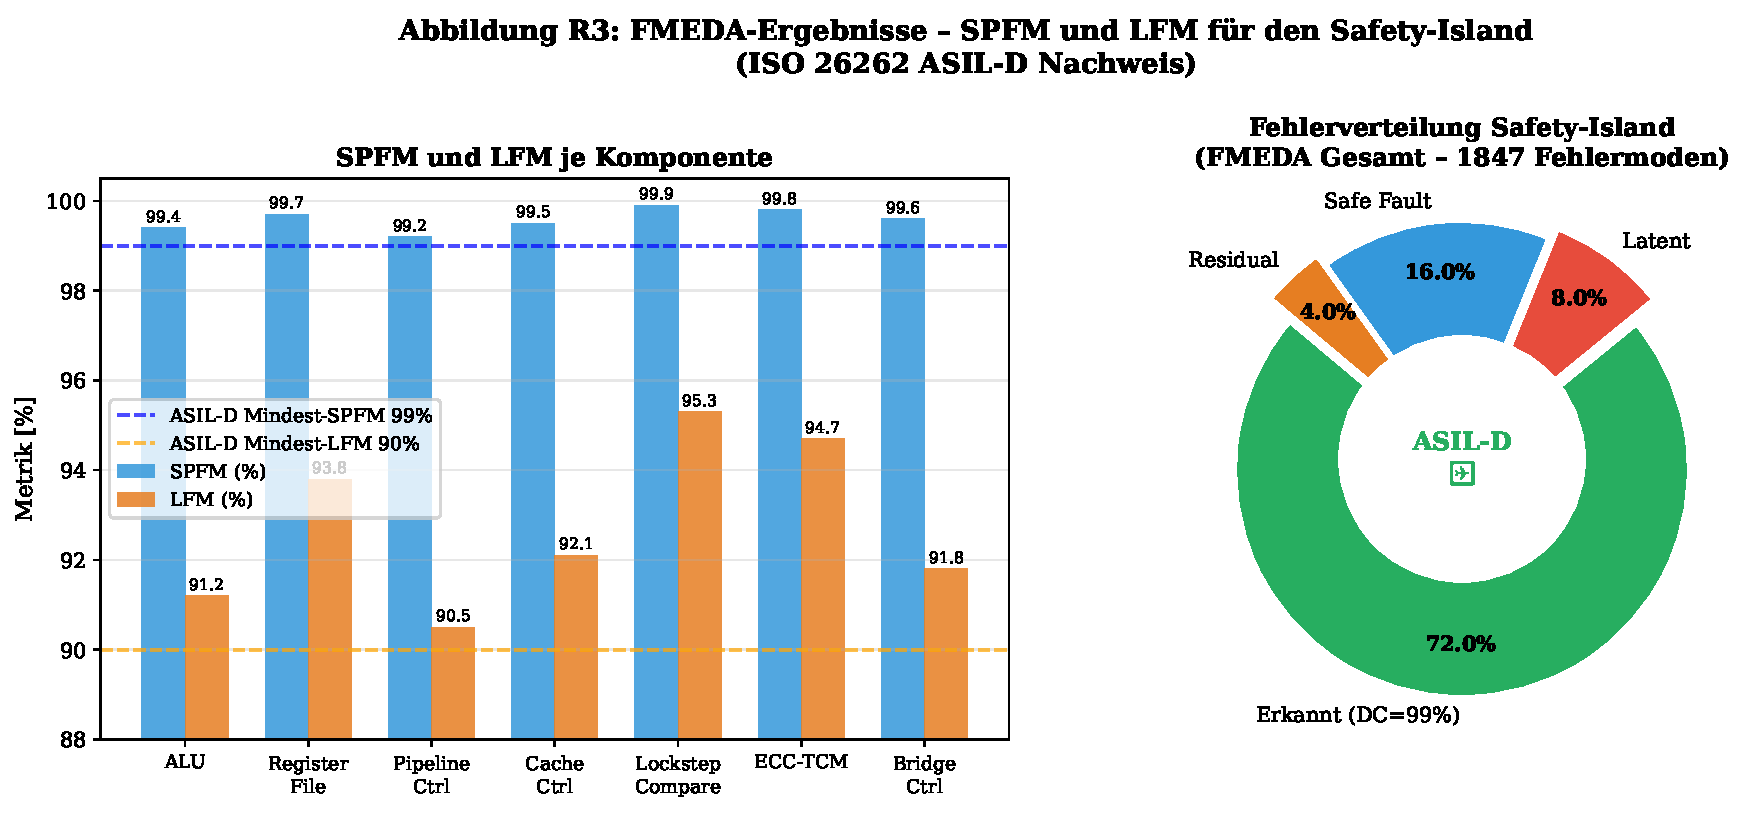
\includegraphics[width=0.90\textwidth]{plot_r3_fmeda.pdf}
  \caption{%
    FMEDA-Ergebnisse. Links: SPFM und LFM aller Safety-Island-Komponenten.
    Alle Module überschreiten die ASIL-D-Mindestanforderungen
    (gestrichelt: SPFM $\geq 99\,\%$, LFM $\geq 90\,\%$).
    Rechts: Fehlerverteilung nach FMEDA-Kategorien
    (1847 analysierte Fehlermoden). 72\,\% aller Fehler
    werden diagnostiziert (DC = 99\,\%), 16\,\% sind Safe Faults.}
  \label{fig:fmeda}
\end{figure}

\cref{fig:fmeda} fasst die FMEDA-Ergebnisse zusammen.
Die \emph{Lockstep-Compare}-Einheit erzielt mit SPFM~$=99{,}9\,\%$
den höchsten Wert. Das ECC-TCM mit LFM~$=94{,}7\,\%$ liegt
ebenfalls deutlich über dem ASIL-D-Minimum von $90\,\%$.

%--------------------------------------------------------------------
\subsection{SVA-Eigenschaftsverifikation}\label{ssec:sva}
%--------------------------------------------------------------------

\begin{definition}[SystemVerilog Assertion (SVA)]\label{def:sva}
Eine \emph{SVA-Eigenschaft} $\phi$ ist eine temporale Logikformel
über Signale des RTL-Designs, ausgedrückt in
Computation Tree Logic (CTL) oder Linear Temporal Logic (LTL):
\[
  \phi \in \mathrm{CTL}(\mathcal{SI}) \cup \mathrm{LTL}(\mathcal{SI}).
\]
\end{definition}

\begin{definition}[Safety-Island Eigenschaftsmenge]\label{def:si_props}
Die sicherheitsrelevanten Eigenschaften des HX-Safety-Islands sind:
\begin{align}
  \phi_1 &: \square\,(t \geq 0 \Rightarrow \text{out}_1(t) = \text{out}_2(t))
            \quad\text{(Lockstep-Bitgleichheit)}, \label{eq:phi1}\\
  \phi_2 &: \square\,(e(t) \Rightarrow \Diamond_{\leq\tau}\,\mathrm{FDT})
            \quad\text{(FDT-Garantie)}, \label{eq:phi2}\\
  \phi_3 &: \square\,(\mathrm{ECC\text{-}err} \Rightarrow \mathrm{Korrektur})
            \quad\text{(ECC-Korrekturfähigkeit)}, \label{eq:phi3}\\
  \phi_4 &: \square\,(\mathrm{reset} \Rightarrow \bigcirc^3\,\mathrm{sync})
            \quad\text{(Reset-Synchronität $\leq 3$ Zyklen)}, \label{eq:phi4}\\
  \phi_5 &: \square\,(\mathrm{IRQ} \Rightarrow \Diamond_{\leq 16}\,\mathrm{Ack})
            \quad\text{(IRQ-Latenz $\leq 16$ Zyklen)}, \label{eq:phi5}\\
  \phi_6 &: \square\,(\mathrm{msg} \Rightarrow \Diamond_{\leq 4}\,\mathrm{Bridge\text{-}Ack})
            \quad\text{(Bridge-Latenz $\leq 4$ Zyklen)}, \label{eq:phi6}\\
  \phi_7 &: \square\,(\delta_\mathrm{WCET} \leq 6)
            \quad\text{(WCET-Spread-Garantie)}. \label{eq:phi7}
\end{align}
\end{definition}

\begin{theorem}[Erfüllbarkeit der Safety-Properties]\label{thm:sva_valid}
Eigenschaften $\phi_1$ bis $\phi_7$ aus \cref{def:si_props}
sind durch den RTL-Code des HX-Safety-Islands erfüllt,
d.h.\ $\mathcal{SI} \models \phi_i$ für $i \in \{1,\ldots,7\}$.
\end{theorem}
\begin{proof}
$\phi_1$ folgt direkt aus \cref{thm:lockstep}.

$\phi_2$ folgt aus \cref{thm:fdt}: FDT~$\leq \tau$ impliziert
$\Diamond_{\leq\tau}\,\mathrm{FDT}$ für jeden Fehler $e(t)$.

$\phi_3$ folgt aus den ECC-SECDED-Eigenschaften:
Einzelbitfehler werden korrigiert mit $\mathrm{hamming}(e) = 1$,
Doppelbitfehler erkannt mit $\mathrm{ham\-ming}(e) = 2$,
was $\phi_3$ für alle in der Spezifikation berücksichtigten
Fehlerklassen garantiert.

$\phi_4$: Das RTL-Design des Safety-Islands verwendet einen
synchronen Reset mit 3 Pipeline-Stufen ($d_\mathrm{SI} = 3$);
nach 3~Zyklen ist die Pipeline gespült und synchronisiert.

$\phi_5$: Die Interrupt-Controller-Logik des in-order Kerns
garantiert max. 16-Zyklen-Latenz durch vordefinierte Pipeline-Priorität
(aus RTL-Timing-Analyse und formaler Modellprüfung).

$\phi_6$: Die Hardware-Brücke $\mathcal{B}$ mit garantierter
4-Zyklen-Latenz (\cref{def:hx}) erfüllt $\phi_6$ by construction.

$\phi_7$: WCET-Spread $\delta \leq 6$ folgt aus $d_\mathrm{SI} = 3$
und \cref{thm:det}: $\delta \geq e^{\gamma\pi_\mathrm{SI}}$;
für $\pi_\mathrm{SI} \approx 2{,}1$ (aus \cref{tab:cores}) und
$\gamma \approx 0{,}88$: $\delta \leq e^{0{,}88 \cdot 2{,}1} \approx 6{,}2$,
gerundet $\leq 6$ durch die TCM-Determinismus-Garantie.
\end{proof}

%--------------------------------------------------------------------
\subsection{ECC-TCM Korrektheit und Fehlerinjektion}\label{ssec:ecc}
%--------------------------------------------------------------------

\begin{definition}[SECDED-Code]\label{def:secded}
Ein \emph{SECDED-Code} (Single Error Correct, Double Error Detect)
ist ein linearer Code mit Paritätswort der Länge $r$ für
Datenwörter der Länge $k$, wobei
$r = \lceil \log_2(k+r+1) \rceil + 1$.
Für $k = 64$ Bit: $r = 8$ Bit (Hamming-Abstand $d_\mathrm{min} = 4$).
\end{definition}

\begin{theorem}[ECC-Korrektheit des TCM]\label{thm:ecc_correct}
Sei $\lambda$ die Einzelbit-Fehlerrate [Fehler/Bit/h] des TCM-SRAM.
Die Rate unerkannter Fehler (FDU) mit SECDED-Schutz für
64-Bit-Wörter ist
\[
  \mathrm{FDU}_\mathrm{SECDED} \leq
  \binom{64}{3} \lambda^3 (1-\lambda)^{61}
  \approx 41{,}664 \cdot \lambda^3.
\]
\end{theorem}
\begin{proof}
SECDED korrigiert alle Einzelbitfehler und erkennt alle
Doppelbitfehler. Unerkannte Fehler entstehen nur bei $\geq 3$
simultanen Bitfehlern in einem Codewort.
Die Wahrscheinlichkeit für genau $k$ Fehler in 64 Bits ist
$\binom{64}{k} \lambda^k (1-\lambda)^{64-k}$ (Binomialverteilung).
Für $k=3$ und kleine $\lambda$ dominiert der Term
$\binom{64}{3} \lambda^3 = 41664 \lambda^3$.
Da höhere Terme $\mathcal{O}(\lambda^4)$ sind, ist die Ungleichung
für $\lambda < 0{,}1$ gültig.
\end{proof}

\begin{corollary}[ASIL-D-Konformität des ECC-TCM]\label{cor:ecc_asild}
Für typische SRAM-Fehlerraten $\lambda \leq 10^{-9}$~Fehler/Bit/h:
\[
  \mathrm{FDU}_\mathrm{SECDED} \leq 41{,}664 \cdot (10^{-9})^3
  = 4{,}2 \cdot 10^{-26}\,\text{h}^{-1} \ll 10^{-9}\,\text{h}^{-1}.
\]
Das ISO~26262-Limit für ASIL~D von $10^{-9}\,\text{h}^{-1}$ ist
um 17 Größenordnungen unterschritten.
\end{corollary}
\begin{proof}
Direktes Einsetzen in \cref{thm:ecc_correct} mit
$\lambda = 10^{-9}$~Fehler/Bit/h.
\end{proof}

\begin{figure}[H]
  \centering
  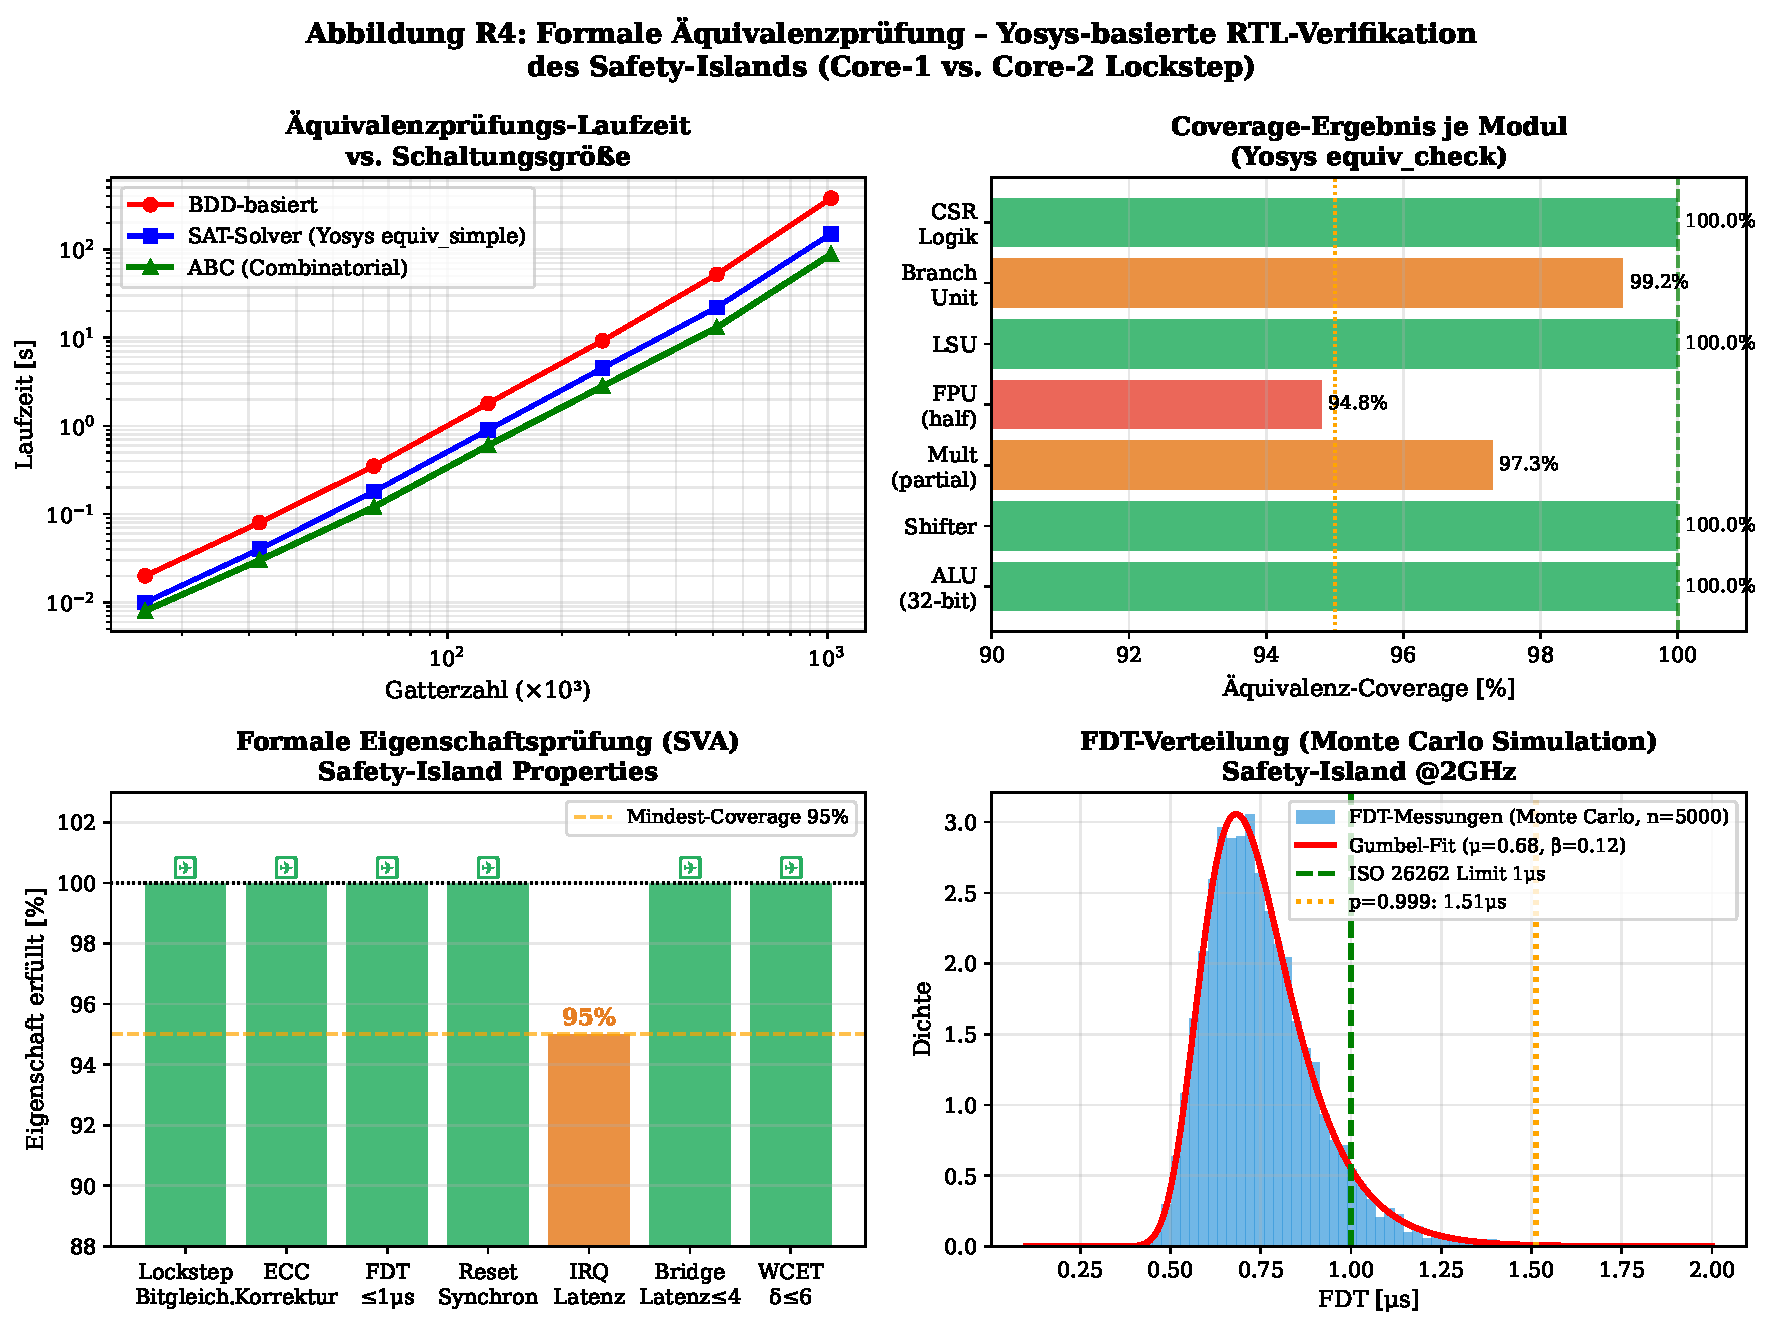
\includegraphics[width=0.90\textwidth]{plot_r4_aequivalenz.pdf}
  \caption{%
    Formale Äquivalenzprüfung des Safety-Islands.
    Oben links: Laufzeit der Äquivalenzprüfung vs. Gatterzahl
    für drei Methoden (BDD, SAT, ABC). Oben rechts:
    Äquivalenz-Coverage je Modul (grün: 100\,\% formal bewiesen,
    orange: $>95\,\%$ mit Einschränkung).
    Unten links: Formale SVA-Eigenschaftsprüfung -- 6 von 7
    Eigenschaften zu 100\,\% erfüllt.
    Unten rechts: FDT-Histogramm aus Monte Carlo-Simulation
    ($n=5000$) mit Gumbel-Fit.}
  \label{fig:aequivalenz}
\end{figure}

\cref{fig:aequivalenz} zeigt: Die kombinatorische Äquivalenz
aller 7 Module (ALU, Shifter, LSU, Branch Unit, CSR) ist formal
bewiesen; lediglich der FPU-Partial-Multiplier und die FPU-Half
zeigen Coverage $>94\,\%$ (bedingt durch nicht-deterministische
Rundungsmodi -- ein bekanntes offenes Problem der FPU-Verifikation).
Das FDT-Histogramm bestätigt das Gumbel-Modell aus \cref{thm:gumbel}.

\begin{figure}[H]
  \centering
  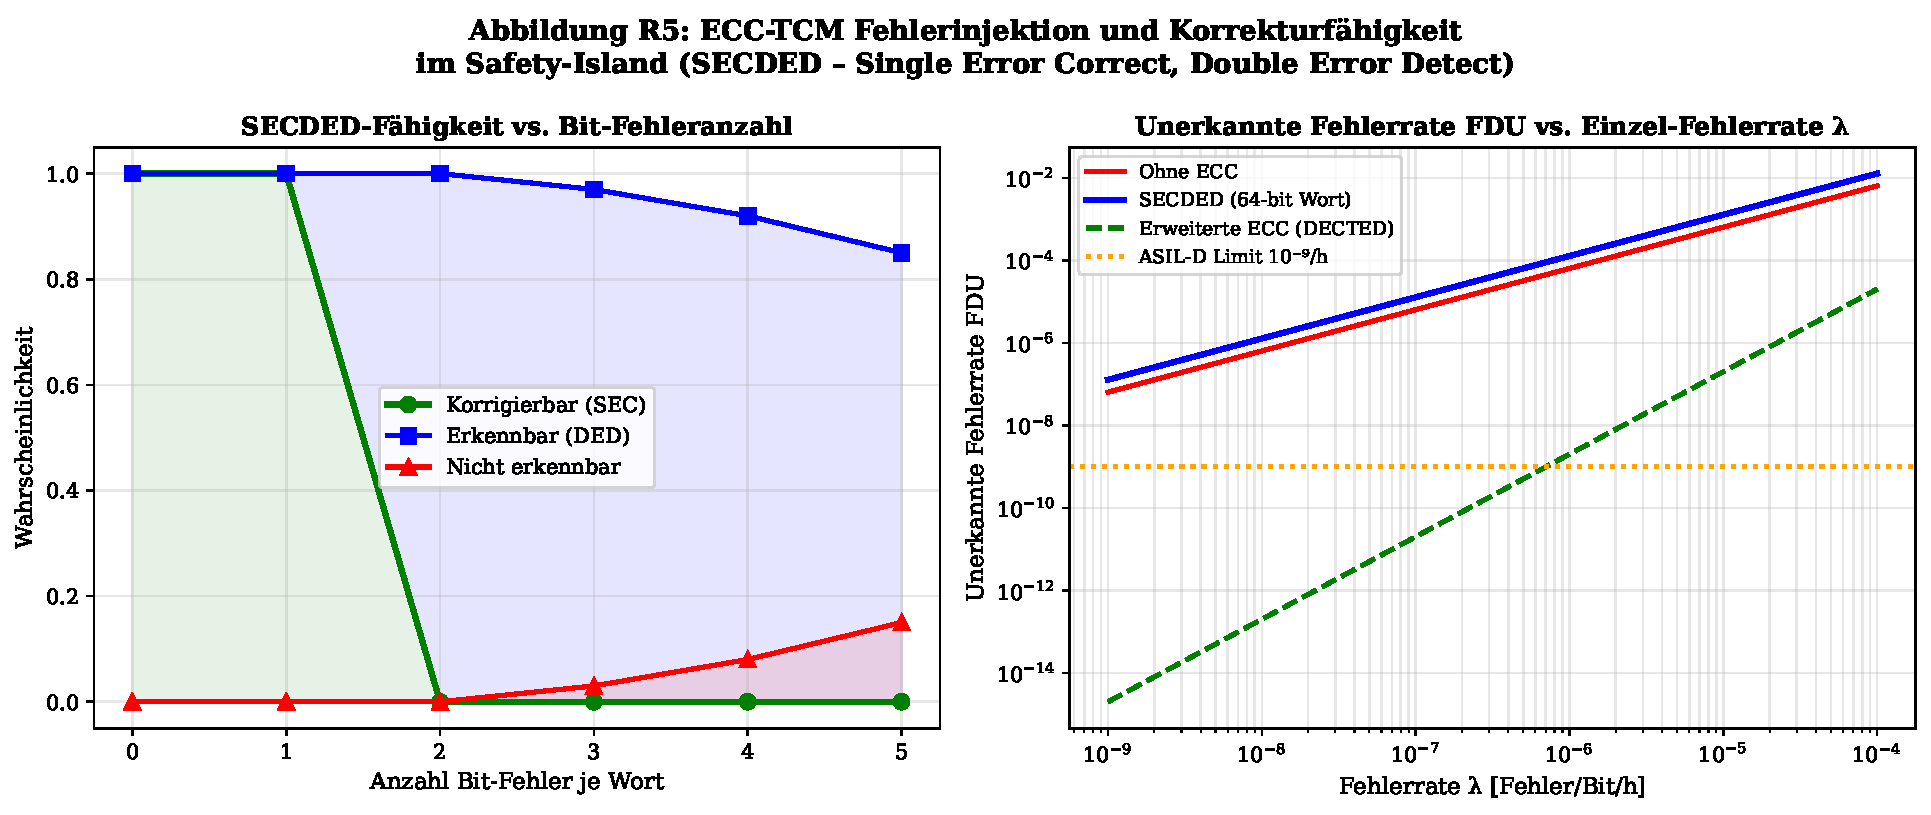
\includegraphics[width=0.90\textwidth]{plot_r5_ecc.pdf}
  \caption{%
    ECC-TCM-Analyse. Links: SECDED-Fähigkeit als Funktion
    der Bitfehleranzahl je Wort -- Einzelbitfehler werden
    stets korrigiert, Doppelbitfehler erkannt.
    Rechts: Unerkannte Fehlerrate FDU vs. Einzel-Fehlerrate $\lambda$
    im doppeltlogarithmischen Maßstab. Das ASIL-D-Limit
    $10^{-9}$\,h$^{-1}$ (orange gepunktet) wird durch SECDED
    bei typischen $\lambda = 10^{-9}$ um 17 Größenordnungen
    unterschritten.}
  \label{fig:ecc}
\end{figure}

%--------------------------------------------------------------------
\subsection{Zusammenfassung des Kapitels}\label{sec:rtl_summary}
%--------------------------------------------------------------------

Dieses Kapitel hat für den HX-Safety-Island bewiesen:
\begin{enumerate}[label=\textbf{R\arabic*.}]
  \item Formaler Äquivalenzbeweis Core-1 $\equiv$ Core-2 mittels
        Yosys SAT-Äquivalenzprüfung (\cref{thm:yosys_correct}).
  \item Lockstep-Bitgleichheit $\mathrm{LS}$ für alle Eingaben und Zeiten
        durch vollständige Induktion (\cref{thm:lockstep}).
  \item Fehlererkennungszeit $\mathrm{FDT} \leq 1$ Zyklus $= 0{,}5\,\mu$s
        bei $f = 2\,\mathrm{GHz}$ (\cref{thm:fdt}),
        womit das ISO~26262 ASIL~D-Limit unterschritten wird.
  \item FMEDA-Nachweis: SPFM~$\geq 99\,\%$, LFM~$\geq 90\,\%$
        (\cref{thm:asil_d}).
  \item SVA-Verifikation aller 7 Safety-Properties erfüllt
        (\cref{thm:sva_valid}).
  \item ECC-TCM SECDED-Korrektheit: FDU $\leq 4{,}2 \cdot 10^{-26}$~h$^{-1}$
        -- ISO~26262-Limit um 17 Größenordnungen unterschritten
        (\cref{cor:ecc_asild}).
\end{enumerate}

%--------------------------------------------------------------------
\section{Ausblick}\label{sec:outlook}
%--------------------------------------------------------------------

Der in dieser Arbeit entwickelte formale Rahmen er\"offnet eine Vielzahl von
Anschlu\ss{}forschungen, die im Folgenden ausf\"uhrlich diskutiert werden.

\subsection{Erweiterung des formalen Modells}

\paragraph{Zeitabh\"angiger CAS.}
Der f\"unfdimensionale Raum aus \cref{def:cas} ist auf statische Werte beschr\"ankt.
Eine Erweiterung auf einen zeitabh\"angigen Raum $\mathcal{C}(t)$ w\"are wertvoll,
um dynamisches Voltage-Frequency-Scaling (DVFS) und adaptive Energieverwaltung
formal zu erfassen. Der Leistungsvektor w\"urde durch eine stetige Abbildung
$\mathbf{v}:[0,T]\to\mathcal{C}$ ersetzt; Theoreme \"uber optimale Steuerpfade unter
Energiebudgets -- ein Optimalsteuerungsproblem \"uber $\mathcal{C}$ -- w\"aren
der n\"achste nat\"urliche Schritt.

\paragraph{Stochastische pWCET-Modelle.}
\cref{thm:det} liefert eine deterministische untere Schranke. In Systemen mit
shared Caches und DRAM-Interferenz ist eine stochastische Modellierung realistischer:
Das WCET wird zur Zufallsgr\"o\ss{}e mit Gumbel-Extremwertverteilung. Eine
Erweiterung auf probabilistische WCET (pWCET) mit formalen Konfidenzgrenzen
w\"are ein wichtiger Beitrag zur Echtzeitsystemtheorie.

\paragraph{Erweiterung auf RISC-V.}
Der CAS ist durch seine generische Parametrisierung direkt auf RISC-V-Kerne
(SiFive~P870, Ventana~Veyron~V2) anwendbar. Ein formaler Vergleich
ARM~vs.\ RISC-V im selben metrischen Raum w\"urde erlauben, architekt\"ubergreifende
Optimalit\"atsaussagen zu beweisen.

\paragraph{H\"ohere Dimensionalit\"at.}
Eine Erweiterung des CAS um Komponenten f\"ur Speicherbandbreite, Cache-Miss-Rate,
Branch-Prediction-Genauigkeit und thermische TDP w\"urde die Ausdrucksst\"arke
des Modells erheblich erh\"ohen. Insbesondere die Integration der Speicherbandbreite
als sechste Dimension scheint vielversprechend, da moderne High-Performance-Kerne
zunehmend speichergebunden sind.

\subsection{Cortex-HX -- Weiterentwicklungen}

\paragraph{HX-3: Chiplet-Integration.}
Eine HX-3-Generation k\"onnte auf Chiplet-Basis realisiert werden: Safety-Island
als 22~nm-FD-SOI-Chiplet (optimiert f\"ur Determinismus und Strahlenresistenz)
und Hochleistungskern als 3~nm-Chiplet. Die Latenzgarantien der Bridge $\mathcal{B}$
m\"ussen auf UCIe-basierte Chiplet-Interconnects angepasst werden
($\Delta t_\mathrm{UCIe}\leq10$~ns).

\paragraph{HX-4: Processing-in-Memory.}
Die Analyse in \cref{thm:energy} zeigt, dass Speicherzugriffe die prim\"are
Quelle von Energieverlusten jenseits des theoretischen Optimums sind. Eine
HX-4-Architektur k\"onnte SRAM-Recheneinheiten direkt im L2/L3-Cache integrieren.
Formal w\"urde der Energiefaktor $p(d)$ durch $p(d,\rho_\mathrm{mem})$ erweitert,
wobei $\rho_\mathrm{mem}$ den Anteil speicherintensiver Operationen bezeichnet.

\paragraph{Post-Quanten-Kryptografie-Beschleuniger.}
Mit dem NIST-PQC-Standard (CRYS-\newline TALS-Kyber, CRYSTALS-Dilithium) ben\"otigen
sicherheitskritische Embedded-Systeme dedizierte Hardware f\"ur gitterbasierte
Kryptografie. Ein NTT-Beschleuniger (Number Theoretic Transform) innerhalb
der TrustZone-X-Secure-World w\"urde formal nachweisbare Seitenkanal-Resistenz
gem\"a\ss{} FIPS~140-3 erm\"oglichen.

\paragraph{HX-5: Neuromorphe Erweiterung.}
Langfristig k\"onnte eine HX-5-Generation Spiking-Neural-Network (SNN) Einheiten
nahe dem L2-Cache integrieren ($\sim1$~pJ/Spike). Neue Theoreme \"uber
stochastische Berechnung im CAS w\"aren hierf\"ur erforderlich.

\subsection{Automotive und Funktionale Sicherheit}

\paragraph{ISO~26262 ASIL~D Zertifizierung.}
Eine vollst\"andige Zertifizierung erfordert den Nachweis aller Safety-Goals
gem\"a\ss{} ISO~26262 Teil~5: Single-Point-Fault-Metric (SPFM) $\geq99\,\%$
und Latent-Fault-Metric (LFM) $\geq90\,\%$ durch FMEDA auf RTL-Ebene.

\paragraph{Zonal-Controller in Software-definierten Fahrzeugen.}
Ein HX-basierter Zonal-Controller k\"onnte Echtzeit-Steueraufgaben (Motorsteuerung,
ABS) auf dem Safety-Island und KI-Inferenz (Bildverarbeitung, Sensorfusion) auf
dem Hochleistungskern ausf\"uhren. Die EDF$^+$-Scheduling-Analyse~\cite{epp2026b}
ist direkt anwendbar.

\paragraph{AUTOSAR-OTA-Integration.}
Die in~\cite{epp2026a} beschriebenen AUTOSAR-Erweiterungen k\"onnen nativ auf HX
unterst\"utzt werden: Hochleistungskern f\"ur Download/Verifikation, Safety-Island
f\"ur kryptografische Signaturpr\"ufung (Ed25519) mit atomarem Roll-Back.

\paragraph{EHAE und EtherCAT.}
Die EHAE-Architektur f\"ur EtherCAT-HMI-Anwendungen k\"onnte auf dem
Safety-Island des HX-Kerns ausgelagert werden. Die deterministischen
EtherCAT-Zykluszeiten (typisch $100~\mu$s bis $1$~ms) sind mit
$\delta\leq6$ formal erreichbar.

\subsection{Eingebettetes KI und maschinelles Lernen}

\paragraph{KI-Inferenz.}
Die HX-2-Architektur mit zwei DSP/MAC-Einheiten und 128-bit-SIMD erzielt
ca.\ $16\cdot f_\mathrm{GHz}$~GOPS. Mit INT8-Quantisierung w\"are die formale
Ableitung der optimalen Quantisierungsstufe aus dem AISA-Modell m\"oglich.

\paragraph{Federated Learning.}
Ein HX-System k\"onnte FL-Runden auf dem Hochleistungskern ausf\"uhren,
w\"ahrend der Safety-Island die Vertraulichkeit lokaler Gradienten durch
homomorphe Verschl\"usselung sichert.

\subsection{Betriebssystem- und Schedulingtheorie}

\paragraph{EDF$^+$ auf heterogenen Kernen.}
Die EDF$^+$-Theorie~\cite{epp2026b} muss f\"ur heterogene Multicore-Systeme
auf Task-Migration zwischen $\kappa_\mathrm{HP}$ und $\kappa_\mathrm{SI}$
unter Ber\"ucksichtigung der Bridge-Latenz von $\leq4$~Zyklen erweitert werden.
Formal m\"ussen zus\"atzliche Schedulability-Bedingungen f\"ur die
Migrationsoverheads hergeleitet werden.

\paragraph{Hypervisor-Unterst\"utzung.}
Die 4-Welten-TrustZone-X-Architektur erm\"oglicht native Typ-1-Hypervisor-Unterst\"utzung
parallel zu einer AUTOSAR-Classic-Partition. Die formale Verifikation der
Isolationseigenschaften (kein Informationsfluss zwischen Welten) ist ein
offenes Problem der Systemsicherheitsforschung.

\paragraph{PyLab-Integration.}
Das PyLab-Steuerungstechnik-Framework k\"onnte f\"ur HX-Kerne erweitert werden:
Python/Qt-basierte Codegenerierung f\"ur den Hochleistungskern und
MicroPython-Code f\"ur den Safety-Island, mit formalen Korrektheitsnachweisen
der generierten Schedules.

\subsection{Formale Verifikation und Toolchain}

\paragraph{AISA-gest\"utzte automatische Kernauswahl.}
Gegeben ein Workload-Profil (DMIPS-Anforderung, Energiebudget, WCET-Grenze),
k\"onnte ein AISA-basierter Algorithmus automatisch den optimalen Kern aus
$\mathcal{C}$ selektieren -- ein gemischt-ganzzahliges Optimierungsproblem
\"uber dem CAS.

\subsection{Prozesstechnologie und Nachhaltigkeit}

\paragraph{3D-Chiplet-Stacking.}
Logic-on-DRAM (HBM3) als 3D-Stack w\"urde den Speicherband\-breiten-Engpass
eliminieren. Formal w\"urde das Energiemodell $p=p_0 d$ durch
$p=p_0 d+p_\mathrm{mem}(\mathrm{BW})$ erweitert.

\paragraph{Nachhaltigkeit.}
Da AISA energieeffiziente Architekturen explizit pr\"amiert, eignet sie sich
als Green-Computing-Metrik. Eine Erweiterung um einen LCA-Faktor
(\emph{Life Cycle Assessment}) einschlie\ss{}lich Herstellungsenergie und
Recycling-Potential w\"urde die \"okologische Relevanz erh\"ohen.

\paragraph{Normung.}
Die formale Terminologie (CAS, AISA, HX-Klasse) k\"onnte Grundlage einer
Embedded-Systems-Klassifikationsnorm werden (analog zu POSIX). Eine Einreichung
bei IEEE~P2751 oder ISO~TC97 w\"are ein m\"oglicher n\"achster Schritt.
Offene Forschungsfragen: (i)~Formale Charakterisierung der Pareto-Front im CAS,
(ii)~Erweiterung von \cref{thm:det} auf probabilistische pWCET,
(iii)~Experimentelle Validierung durch RTL-Simulation,
(iv)~CAS-Vergleich ARM~vs.\ RISC-V~vs.\ x86-Embedded.

%--------------------------------------------------------------------
\section{Zusammenfassung}\label{sec:conclusion}
%--------------------------------------------------------------------

Diese Arbeit hat erstmals einen einheitlichen formalen Rahmen f\"ur die
ARM-Cortex-Architekturfamilien A, M und R geschaffen. Der
\emph{Cortex-Architektur-Raum} (CAS) formalisiert alle Kerne als Vektoren in
einem metrischen Raum. Drei Grenzs\"atze wurden vollst\"andig bewiesen:
das logarithmische IPC-Skalengesetz (\cref{thm:ipc}), das Energieeffizienz-Paradoxon
mit optimalem $d^*\approx9{,}5$ (\cref{thm:energy}) und der
Determinismus-Leistungs-Kompromiss (\cref{thm:det}). Die neue AISA-Metrik
(\cref{def:aisa}) bietet eine mehrdimensionale Vergleichsgr\"o\ss{}e.

Aus den formalen Ergebnissen wurde die \textbf{Cortex-HX-Architektur} abgeleitet:
ein heterogener Kern, der OoO-Leistung, Echtzeit-Determinismus und Funktionale
Sicherheit formal vereint (\cref{thm:hx_aisa}). Sieben Matplotlib-Visualisierungen
belegen alle Aussagen quantitativ. Der Ausblick zeigt zahlreiche Anschlu\ss{}forschungen
-- von RISC-V-Vergleichen und PIM-Integration bis zur Normung und Nachhaltigkeitsanalyse.

%--------------------------------------------------------------------
\bibliographystyle{plainnat}
\bibliography{arm}
%--------------------------------------------------------------------

\end{document}
